%----------------------------------------------------------------------------------------
%    PACKAGES AND THEMES
%----------------------------------------------------------------------------------------

\documentclass[aspectratio=169,xcolor=dvipsnames]{beamer}
%\usepackage{siunitx}
\usetheme{SimplePlus}
% References to sections, lemmas, theorems, etc.
\newcommand{\sref}[1]{\S\ref{#1}}
\newcommand{\fref}[1]{Figure~\ref{#1}}
% Abbreviations.
\def\etal.{\emph{et al.}}
\newcommand{\SL}{Separation Logic\xspace}
\newcommand{\spacelang}{SpaceLang\xspace}
\let\ar\rightarrow
\newcommand{\iProp}{\mathit{iProp}}
\newcommand{\lc}{$\lambda$-calculus\xspace}

% I have hesitated between "logical heap" (Dreyer et al.'s terminology)
% and "conceptual heap".
\newcommand{\logical}{logical\xspace}
\newcommand{\logically}{logically\xspace}
\newcommand{\Logical}{Logical\xspace}
%types
\newcommand{\tlfoff}[1]{\kw{pml4off}:#1}
\newcommand{\tltoff}[1]{\kw{pdpoff}:#1}
\newcommand{\tltwoff}[1]{\kw{pdoff}:#1}
\newcommand{\tlooff}[1]{\kw{ptoff}:#1}
\newcommand{\tpgoff}[1]{\kw{pageoff}:#1}
\newcommand{\lfoff}{\kw{pml4off}}
\newcommand{\ltoff}{\kw{pdpoff}}
\newcommand{\ltwoff}{\kw{pdoff}}
\newcommand{\looff}{\kw{ptoff}}
\newcommand{\pgoff}{\kw{pageoff}}
\newcommand{\crt}{\kw{cr3}}
\newcommand{\lt}{\kw{pdp}}
\newcommand{\ltw}{\kw{pd}}
\newcommand{\lo}{\kw{pt}}
\newcommand{\pg}{\kw{page}}
\newcommand{\tlf}[1]{\kw{cr3}:#1}
\newcommand{\tlt}[1]{\kw{pdp}:#1}
\newcommand{\tltw}[1]{\kw{pd}:#1}
\newcommand{\tlo}[1]{\kw{pt}:#1}
\newcommand{\tpg}[1]{\kw{page}:#1}
%modal assertions
\newcommand{\modalPs}[1]{\vec#1}
\newcommand{\modalP}{P}
\newcommand{\modalQ}{Q}
\newcommand{\modaldefper}[2]{@[#1]\;\square\;#2}
\newcommand{\outsidemodaldefper}[2]{\square \; @[#1]\; #2}
\newcommand{\modaldef}[2]{@[#1]\; #2 }
\newcommand{\modaldefunfold}[2]{ #2 \; #1}
\newcommand{\modalstar}[2]{#1 \star #2}

% Assertions.
\newcommand{\qfracone}{\kw{1}}
\newcommand{\qfracfot}{\kw{q}/512}
\newcommand{\qfracfots}{\kw{q}/512^{2}}
\newcommand{\qfracfotss}{\kw{q}/512^{4}}
\newcommand{\qfracfotsss}{\kw{q}/512^{8}}

\newcommand{\qfrac}{\kw{q}}
\newcommand{\qfractw}{\kw{q}/2}
\newcommand{\qfract}{\kw{q}/3}
\newcommand{\qfracf}{\kw{q}/4}
\newcommand{\naddr}{\kw{a}}
\newcommand{\vaddr}{\kw{va}}
\newcommand{\vpts}{\kw{v}}
\newcommand{\ppts}{\kw{p}}
\newcommand{\rpts}{\kw{r}}
\newcommand{\pfpointsto}[4]{#1\mapsto_{#4}\{#3\}\;#2}
\newcommand{\ppointsto}[3]{#1\mapsto_{#3}\;#2}
\newcommand{\npointsto}[4]{#1 / #2 \mapsto_{#4}\;#3}

\newcommand{\nfpointsto}[5]{#1\sim#2 \mapsto_{#5}\{#4\}\;#3}
\newcommand{\maskfour}{\textsf{l4M52}}
\newcommand{\maskfouroff}{\textsf{l4off}}
\newcommand{\maskthree}{\textsf{l3M52}}
\newcommand{\maskthreeoff}{\textsf{l3off}}
\newcommand{\masktwo}{\textsf{l2M52}}
\newcommand{\masktwooff}{\textsf{l2off}}
\newcommand{\maskone}{\textsf{l1M52}}
\newcommand{\maskoneoff}{\textsf{l1off}}
%\nfpointsto{\mask\vaddr\ft\rtv}{\mask\vaddr\tw\rtv}\entryf\qone\naddr 
\newcommand{\mask}[3]{(#2\; #1 \; #3)}
\newcommand{\ft}{52}
\newcommand{\tw}{12}
\newcommand{\pointsto}{\mapsto}
\newcommand{\mystackrel}[2]{#2_{#1}}
\newcommand{\fpointsto}[1]{\mathrel{\mystackrel{#1}{\mapsto}}}
\newcommand{\pointedby}{\mapsfrom}
\newcommand{\vfpointedby}[1]{\mathrel{\mystackrel{#1}{\mapsfrom}}}
\newcommand{\vpointedby}{\mathrel{\mapsfrom}}
\newcommand{\mydagger}{\mathord{\dagger}}
\renewcommand{\ddag}{\mydagger\kern-0.8mm\mydagger}
\newcommand{\ddagsingleton}[1]{\ddag\{#1\}}
% \newcommand{\ocloud}[3]{\tensor*[_{#3}]{\text{\faCloud}}{^{#2}_{#1}}}
\newcommand{\ocloud}[3]{#3\;\text{\faCloud}^{#2}\,#1}
\newcommand{\cloud}[2]{\ocloud{#1}{#2}{#1}}
\newcommand{\pure}[1]{#1}
% Reference counting.
\newcommand{\rcpointedby}{\mathrel{\mapsfrom}}
\newcommand{\rcvpointedby}{\mathrel{\mapsfrom}}
\newcommand{\rcvfpointedby}[1]{\mathrel{\mapsfrom}_{#1}}
\newcommand{\nmaster}{m}
\newcommand{\nv}{n}
% Central invariant
\newcommand{\centralinvariant}{I}
\newcommand{\generalentry}{\textsf{ent}}
\newcommand{\entryf}{\textsf{l4e}}
\newcommand{\entrytr}{\textsf{l3e}}
\newcommand{\entrytw}{\textsf{l2e}}
\newcommand{\entryo}{\textsf{l1e}}
\newcommand{\crthree}{\textsf{CR3}}
\newcommand{\paddr}{\textsf{pa}}
\newcommand{\vsome}{\_}
\newcommand{\vpage}{\textsf{v}}
% Fonts.
\newcommand{\kw}[1]{\mathsf{#1}}

% Metavariables:

% Locations.
\newcommand{\pageptstosum}[2]{(#1+#2)}
\newcommand{\lvlsum}[2]{(#1+8*#2)}
\newcommand{\lvlbor}[1]{(#1 | \kw{w0}_{3})}
\newcommand{\Locsx}{\mathcal{W}_{16}}
\newcommand{\locsx}{\kw{w}_{16}}
\newcommand{\Locsz}{\mathcal{W0}_{16}}
\newcommand{\locsz}{\kw{w0}_{16}}

\newcommand{\Locn}{\mathcal{W}_{9}}
\newcommand{\locn}{\kw{w}_{9}}

\newcommand{\Loctw}{\mathcal{W}_{12}}
\newcommand{\loctw}{\kw{w}_{12}}
\newcommand{\Locsf}{\mathcal{W}_{64}}
\newcommand{\locsf}{\kw{w}_{64}}
\newcommand{\Locft}{\mathcal{W}_{52}}
\newcommand{\locft}{\kw{w}_{52}}

\newcommand{\rvsrc}{\kw{rv}_{\textsf{src}}}
\newcommand{\rgsrc}{\kw{r}_{\textsf{src}}}
\newcommand{\rv}{\kw{rv}}
\newcommand{\rg}{\kw{r}}
\newcommand{\rvdst}{\kw{rv}_{\textsf{dst}}}
\newcommand{\rgdst}{\kw{r}_{\textsf{dst}}}

\newcommand{\mvsrc}{\kw{rv}_{\textsf{src}}}
\newcommand{\mgsrc}{\kw{r}_{\textsf{src}}}
\newcommand{\mv}{\kw{rv}}
\newcommand{\mg}{\kw{r}}
\newcommand{\mvdst}{\kw{rv}_{\textsf{dst}}}
\newcommand{\mgdst}{\kw{r}_{\textsf{dst}}}

\newcommand{\Loc}{\mathcal{W}_n}
\newcommand{\loc}{\kw{w}_n}
\newcommand{\regset}{\kw{greg}}
\newcommand{\regvaltype}{\kw{regval}}
\newcommand{\reg}{\kw{r}}
\newcommand{\regval}{\kw{rv}}
% Formal parameters.
\newcommand{\xs}{\mathit{xs}}
% Assertions.
\newcommand{\pre}{\Phi}
\newcommand{\post}{\Psi}
\newcommand{\midpoint}{\chi}
% Fractions.
\newcommand{\ql}{p}
\newcommand{\qv}{q}
\newcommand{\qw}{q'}
% A multiset of locations.
\newcommand{\lsv}{L}
\newcommand{\lsw}{L'}
% A set of locations.
\newcommand{\locs}{D}
\newcommand{\antecedents}{P}

% Metalevel conditional.
% \newcommand{\metaif}[3]{\text{\it if $#1$ then $#2$ else $#3$}}
\newcommand{\metaif}[3]{#1 \mathrel{?} #2 : #3}

% Values.
\newcommand{\val}{v}
\newcommand{\vals}{\vec\val}
\newcommand{\wal}{v'}
\newcommand{\vunit}{()}
\newcommand{\vk}{k}
\newcommand{\vcode}[2]{\lambda#1.#2}
\newcommand{\vars}{\vec\var}

% LValues.
\newcommand{\lval}{\varrho}
\newcommand{\var}{x}
\newcommand{\sloc}{c}
\newcommand{\src}{r}
\newcommand{\dst}{s}
\newcommand{\dsts}{\vec\dst}
\newcommand{\lvals}{\vec\lval}

\newcommand{\ofs}{\mathit{o}}
\newcommand{\maddr}{\kw{maddr}}
\newcommand{\offs}{\kw{offset}}
% Instructions.
\newcommand{\deref}{\mathord{*}}
\newcommand{\assign}{=}
\newcommand{\instr}{i}
\newcommand{\mvrr}{\kw{mvrr}}
\newcommand{\mvrmb}{\kw{mvrmb}}
\newcommand{\mvrmo}{\kw{mvrmo}}
\newcommand{\mvmrb}{\kw{mvmrb}}
\newcommand{\mvmro}{\kw{mvmro}}
\newcommand{\instrexpr}{\kw{ie}}
\newcommand{\instrs}{\ensuremath{\vec\instr}}
\newcommand{\iskip}{\ensuremath{\kw{skip}}}
\newcommand{\iseq}[2]{\ensuremath{#1; #2}}
\newcommand{\ising}[1]{\kw{sexec} (#1)}
\newcommand{\icall}[2]{\deref#1(#2)}
\newcommand{\ialloc}[2]{\deref#1 \assign \kw{alloc}\;#2}
\newcommand{\iload}[3]{\deref#1 \assign [\deref#2+#3]}
\newcommand{\istore}[3]{[\deref#1+#2] \assign \deref#3}
\newcommand{\iloceq}[3]{\deref#1 \assign (\deref#2 == \deref#3)}
\newcommand{\iconst}[2]{\deref#1 \assign #2}
\newcommand{\imove}[2]{\deref#1 \assign \deref#2}
\newcommand{\ialloca}[2]{\kw{alloca}\,#1\,\kw{in}\,#2}
\let\iallocaactive\ialloca
\newcommand{\ifork}[3]{\kw{fork}\,\deref#1\,\kw{as}\,#2\,\kw{in}\,#3}

%mov instructions

\newcommand{\movctl}{\kw{movctl}}
\newcommand{\imreg}{\kw{imreg}}
\newcommand{\amode}{\kw{amode}}
\newcommand{\amodeb}[1]{\kw{amode}  #1}
\newcommand{\amodeo}[2]{\kw{amode} = #1 + #2}
\newcommand{\imov}[3]{#1 \; #2 \; #3}
% Blocks.
\newcommand{\blk}{b}
\newcommand{\btuple}[1]{#1}
\newcommand{\bcell}[1]{\langle#1\rangle}
\newcommand{\bdeallocated}{\text{\normalfont\footnotesize\faBolt}}
\newcommand{\sz}[1]{\mathit{size}(#1)}
\newcommand{\replicate}[2]{#2^{#1}}
\newcommand{\pointers}[1]{\mathit{pointers}(#1)}

% Stores.
\newcommand{\storereg}{\sigma.\mathcal{R}}
\newcommand{\storemem}{\sigma.\mathcal{M}}
\newcommand{\storememstar}[1]{\sigma.\mathcal{M}^{*[#1]}}
\newcommand{\store}{\sigma}
\newcommand{\storeregprime}{\sigma'.\mathcal{R}}
\newcommand{\storememprime}{\sigma'.\mathcal{M}}
\newcommand{\storememprimestar}[1]{\sigma'.\mathcal{M}^{*[#1]}}

\newcommand{\storeprime}{\sigma'}

\newcommand{\logicalstore}{\theta}
\newcommand{\maxsize}{S}
% \newcommand{\valid}[1]{\text{$#1$ is valid}}
\newcommand{\valid}[1]{\sz{#1}\leqmaxsize}
\newcommand{\available}[1]{\mathit{available}(#1)}
\newcommand{\closed}[1]{\text{$#1$ is closed}}
\newcommand{\related}[2]{#1\approx#2}

% Predecessor maps (\pi).
\newcommand{\predstore}{\pi}
\newcommand{\phinvariant}[2]{#1\bowtie#2}

% Evaluation contexts.
\newcommand{\ectx}{K}
\newcommand{\hole}{[]}
\newcommand{\efill}[2]{#1[#2]}

% Semantics.
\newcommand{\subst}[2]{[#2/#1]}
\newcommand{\readlval}[3]{#2(#1)=\bcell{#3}}
\newcommand{\writelvalsidecondition}[4]{
  #3(#1) = \bcell{\_}
}
\newcommand{\writelvalmaincondition}[4]{
  #4 = \mupd{#1}{\bcell{#2}}{#3}
}
% fp: I would like to hide the side condition in \writelval,
%     for greater clarity, but the reviewers want to see it.
% fp: let me invent a notation to indicate that we overwrite
%     a stack cell with a stack cell.
\newcommand{\writelval}[4]{
  #4 = \langle #1 := #2 \rangle #3
}

\newcommand{\sexec}[4]{\kw{sexec}\(#1 #2 #3 #4\)}
\newcommand{\headstep}{\longrightarrow}
\newcommand{\cfg}[2]{#1\;/\;#2}
\newcommand{\hs}[4]{\cfg{#1}{#2}\headstep\cfg{#3}{#4}}
\newcommand{\hsfork}[5]{\cfg{#1}{#2}\headstep\cfg{#3}{#4}}
\newcommand{\hsforknl}[5]{\begin{array}{@{}r@{}}\cfg{#1}{#2}\headstep\cfg{#3}{#4}\end{array}}
\newcommand{\hsnostore}[2]{\hs{#1}\store{#2}\store}
% \newcommand{\gc}[2]{#1\mathrel{\smash{\stackrel{\mathit{gc}}{\longrightarrow}}}#2}
\newcommand{\gcSymbol}{\text{\normalfont\footnotesize\faTrashO}}
\newcommand{\gc}[2]{#1\mathrel{\gcSymbol}#2}
\newcommand{\headstepgc}{\mathrel{\;\gcSymbol\!\!\longrightarrow\,}}
\newcommand{\hsgc}[4]{\cfg{#1}{#2}\headstepgc\cfg{#3}{#4}}
\newcommand{\hsgcfork}[5]{\cfg{#1}{#2}\headstepgc\cfg{#3}{#4}}

% Length of an array or list.
\newcommand{\alen}[1]{\mathord\mid#1\mathord\mid}

% Triples.
\newcommand{\varray}[1]{\begin{array}{@{}c@{}}#1\end{array}}
\newcommand{\starvarray}[1]{\bgroup\renewcommand{\star}{\\}\varray{#1}\egroup}
\newcommand{\BRACE}[1]{\left\{#1\right\}}
\newcommand{\BRACEvarray}[1]{\BRACE{\varray{#1}}}
\newcommand{\BRACEstarvarray}[1]{\BRACE{\starvarray{#1}}}
\newcommand{\triple}[3]{\{#1\}\;#2\;\{#3\}}
\newcommand{\atriple}[3]{\triple{#1}{&#2&}{#3}}
\newcommand{\vtriple}[3]{\varray{\{#1\}\\#2\\\{#3\}}}
\newcommand{\bigvtriple}[3]{\varray{\BRACEvarray{#1}\\#2\\\BRACEvarray{#3}}}
\newcommand{\bightriplehskip}{\;}
\newcommand{\bightriple}[3]{\BRACEstarvarray{#1}\bightriplehskip#2\bightriplehskip\BRACEstarvarray{#3}}
\newcommand{\bightriplex}[4]{\BRACEstarvarray{#1}\bightriplehskip#2\bightriplehskip\BRACE{\exists#3.\;\starvarray{#4}}}
\newcommand{\bigsupd}[2]{\BRACEstarvarray{#1}\supd\BRACEstarvarray{#2}}
% WP.
\renewcommand{\wp}[2]{\mathit{wp}\;#1\;#2}

% Iris connectives.
% \renewcommand{\star}{\ast}
\let\ordinarystar\star
\DeclareMathOperator*{\Sep}{\scalerel*{\ast}{\sum}}
\newcommand{\bigast}[2]{\mathop{\textstyle\Sep}\limits_{#1}\,#2}
\let\ordinarybigast\bigast
\newcommand{\later}{\triangleright\;}

\newcommand{\logequiv}{\;\equiv\;}
\newcommand{\supd}{\Rrightarrow_\centralinvariant}
\newcommand{\fupd}{\Rrightarrow}
\let\ordinarysupd\supd
\newcommand{\iFalse}{\mathit{False}}
\newcommand{\iTrue}{\mathit{True}}

% Sets.
\newcommand{\singleton}[1]{\{#1\}}
\newcommand{\dom}[1]{\mathit{dom}(#1)}

% Multisets.
\newcommand{\multiplicity}[2]{#1 \mathop{\text{\small\$}} #2}
\newcommand{\cardinal}[1]{|#1|}
% Number of occurrences of a value in a list of values.
\newcommand{\valoccs}[2]{#1 \mathop{\$} #2}

% Maps.
\newcommand{\singletonMap}[2]{[#1 := #2]}
\newcommand{\mupd}[2]{[#1 := #2]} % update at an existing location
\newcommand{\mext}[2]{[#1 \mathbin{+\!\!=} #2]} % update at a new location

% Names of some reasoning rules.
\newcommand{\JoinPointsto}{Join$\mapsto$}
\newcommand{\JoinPointedBy}{Join$\mapsfrom$}
\newcommand{\CovPointedBy}{Covariance$\mapsfrom$}
\newcommand{\ConfrontMapstoMapsfrom}{Confront$\mapsto\mapsfrom$}
\newcommand{\ConfrontDagMapsfrom}{Confront$\ddag\mathord{\mapsfrom}$}
\newcommand{\ZeroDiams}{Zero$\diamond$}
\newcommand{\JoinDiams}{Join$\diamond$}
\newcommand{\ZeroDag}{Zero$\ddag{}$}
\newcommand{\JoinDag}{Join$\ddag{}$}

\newcommand{\mathsmash}[1]{\ensuremath{\smash{#1}}}

% ------------------------------------------------------------------------------

% Macros for the list copy example.
\newcommand{\crval}{\kw{cr3val}}
\newcommand{\plusaddr}[2]{#1 + #2}
%variable names

% Variable names.

\newcommand{\listcopy}{\textit{copy}}
\newcommand{\self}{\textit{self}\,}
\newcommand{\destination}{\textit{dst}}
\newcommand{\source}{\textit{src}}
\newcommand{\etiquette}{\textit{tag}}
\newcommand{\head}{\textit{head}}
\newcommand{\tail}{\textit{tail}}
\newcommand{\res}{\destination'}
\newcommand{\callee}{\textit{f}\,}
% A logical list of values:
\newcommand{\logval}{\mathit{v}}
\newcommand{\loglist}{\mathit{vs}}
% isList.
\newcommand{\isListName}{\textit{isList}}
\newcommand{\isList}[2]{\isListName\;#1\;#2}
% Logical lists.
\newcommand{\lognil}{[]}
\newcommand{\logcons}[2]{#1 :: #2}
\newcommand{\loglistbrackets}[1]{[#1]}

% ------------------------------------------------------------------------------

% Macros for the stack example.

\newcommand{\stackcreate}{\textit{create}}
\newcommand{\stackpush}{\textit{push}}
\newcommand{\stackpop}{\textit{pop}}
\newcommand{\isStack}[2]{\textit{isStack}\;#1\;#2}
\newcommand{\stack}{\textit{stack}}
\newcommand{\elem}{\textit{elem}}
\newcommand{\vns}{\mathit{vns}}
\newcommand{\nonreccallee}{\ensuremath{f}}

\newcommand{\coq}{\textsc{Coq}\xspace}
\newcommand{\HyLL}{\textsc{HyLL}\xspace}
\newcommand{\BI}{\textsc{BI}\xspace}
\newcommand{\BBI}{\textsc{BBI}\xspace}
\newcommand{\HyBBI}{\textsc{HyBBI}\xspace}
\newcommand{\iris}{\textsc{Iris}\xspace}

\usepackage{etoolbox}
\usepackage{graphicx}


\usepackage{tikz}
\usepackage{hyperref}
\usepackage{amsmath,amssymb,mathpartir,iris}
\usepackage{stmaryrd} % for \llbracket and \rrbracket

\usepackage{graphicx} % Allows including images
\usepackage{booktabs} % Allows the use of \toprule, \midrule and \bottomrule in tables
\usepackage{xcolor}
\usepackage{listings}
\newcommand{\assert}[1]{\{#1\}}
\usepackage[skins,theorems]{tcolorbox}
\tcbset{highlight math style={enhanced,
  colframe=red,colback=white,arc=0pt,boxrule=1pt}}
  
\usetikzlibrary{automata}
  \usetikzlibrary{
                shapes.multipart
                }
\usetikzlibrary{arrows,positioning,calc,backgrounds,positioning,fit,shapes,snakes,quotes,graphs}
% Thanks to Alex Kocurek's "A Quick TikZ Guide for Modal Logicians"
% http://www.actual.world/resources/tex/doc/TikZ.pdf
\tikzset{
modal/.style={>=stealth',shorten >=1pt,shorten <=1pt,auto,node distance=2.0cm,
semithick},
world/.style={circle,draw,minimum size=1cm,fill=gray!15},
point/.style={circle,draw,inner sep=0.5mm,fill=black},
reflexive above/.style={->,loop,looseness=7,in=120,out=60},
reflexive below/.style={->,loop,looseness=7,in=240,out=300},
reflexive left/.style={->,loop,looseness=7,in=150,out=210},
reflexive right/.style={->,loop,looseness=7,in=30,out=330}
}
\tikzset{
modalw/.style={font=\tiny,>=stealth',shorten >=1pt,shorten <=1pt,auto,node distance=0.8cm,
semithick},
world/.style={circle,draw,minimum size=0.75cm,fill=gray!15},
point/.style={circle,draw,inner sep=0.5mm,fill=black},
reflexive above/.style={->,loop,looseness=7,in=120,out=60},
reflexive below/.style={->,loop,looseness=7,in=240,out=300},
reflexive left/.style={->,loop,looseness=7,in=150,out=210},
reflexive right/.style={->,loop,looseness=7,in=30,out=330}
}
 \tikzstyle{background}=[circle split,
                                                    fill=gray!10,
                                                    inner sep=0.0001cm,
                                                    rounded corners=5mm]
 \tikzstyle{backgrounddiamond}=[rectangle,
                                                    fill=gray!10,
                                                    inner sep=0.2cm,
                                                    rounded corners=5mm]

\tikzstyle{background1}=[rectangle,
                                                    fill=darkgray!30,
                                                    inner sep=0.2cm,
                                                    rounded corners=5mm]

\tikzstyle{background2}=[rectangle,
                                                    fill=gray!60,
                                                    inner sep=0.2cm,
                                                    rounded corners=5mm]



\definecolor{mGreen}{rgb}{0,0.6,0}
\definecolor{mGray}{rgb}{0.5,0.5,0.5}
\definecolor{mPurple}{rgb}{0.58,0,0.82}
\definecolor{backgroundColour}{rgb}{0.95,0.95,0.92}
\lstdefinestyle{CStyleNum}{
    backgroundcolor=\color{backgroundColour},   
    commentstyle=\color{mGreen},
    keywordstyle=\color{magenta},
    numberstyle=\tiny\color{mGray},
    stringstyle=\color{mPurple},
    basicstyle=\scriptsize,
    breakatwhitespace=false,         
    breaklines=true,                 
    captionpos=b,                    
    keepspaces=true,                 
   % numbers=left,                    
   % numbersep=5pt,                  
    showspaces=false,                
    showstringspaces=false,
    showtabs=false,                  
   % tabsize=2,
    language=C
}
%,
        \lstdefinestyle{CStyleNumEmph}{
    backgroundcolor=\color{backgroundColour},   
    commentstyle=\color{mGreen},
    keywordstyle=\color{magenta},
    numberstyle=\tiny\color{mGray},
    stringstyle=\color{mPurple},
    basicstyle=\scriptsize,
    breakatwhitespace=false,         
    breaklines=true,                 
    captionpos=b,                    
    keepspaces=true,                 
   % numbers=left,                    
   % numbersep=5pt,                  
    showspaces=false,                
    showstringspaces=false,
    showtabs=false,                  
   % tabsize=2,
    language=C,
    \lstset{emph={P2V, next_virt_addr, next_phys_addr},emphstyle=\textbf}
}
\lstdefinestyle{CStyle}{
    backgroundcolor=\color{backgroundColour},   
    commentstyle=\color{mGreen},
    keywordstyle=\color{magenta},
    numberstyle=\tiny\color{mGray},
    stringstyle=\color{mPurple},
    basicstyle=\scriptsize,
    breakatwhitespace=false,         
    breaklines=true,                 
    captionpos=b,                    
    keepspaces=true,                 
    numbers=left,                    
    numbersep=5pt,                  
    showspaces=false,                
    showstringspaces=false,
    showtabs=false,                  
    tabsize=2,
    language=C
}
\newcommand{\sumwalkabsent}{
  \ownGhost\gammaPred{\authfrag{\singletonMap{\texttt{entry+KERNBASE}}{(\textsf{qfrac}, \textsf{entry})}}}
}

\newcommand{\gammaPred}{\delta}
\newcommand{\gammaPreds}{\delta\textsf{s}}
\newcommand{\rtv}{\textsf{rtv}}
\newcommand{\qone}{\texttt{q1}}
\newcommand{\qtwo}{\texttt{q2}}
\newcommand{\qthree}{\texttt{q3}}
\newcommand{\qfour}{\texttt{q4}}

\newcommand{\sumwalkabs}[3]{
  \ownGhost\gammaPred{\authfrag{\singletonMap{#1}{(#2, #3)}}}
}

\newcommand{\sumapaces}[2]{
  \ownGhost\gammaPreds{\authfrag{\singletonMap{#1}{#2}}}
}
\newcommand{\ptableabswalk}[1]{\mathcal{A}\textsf{bsPTableWalk}(#1)}
\newcommand{\ptablestore}{\theta}
\newcommand{\ventry}{\texttt{entry + KERNBASE}}
\newcommand{\entry}{\texttt{entry}}
\newcommand{\qfraczero}{\textsf{qfrac}}
\newcommand{\true}{\textsf{true}}
\tikzstyle{boxedassert_border} = [sharp corners,line width=0.2pt]
\NewDocumentCommand \boxedassertpv {O{} m o}{%
	\tikz[baseline=(m.base)]{
		%	  \node[rectangle, draw,inner sep=0.8pt,anchor=base,#1] (m) {${#2}\mathstrut$};
		\node[rectangle,inner sep=1.5pt,outer sep=0.2pt,anchor=base] (m) {${\,#2\,}\mathstrut$};
		\draw[#1,boxedassert_border] ($(m.south west)$) rectangle ($(m.north east)$);
	}\IfNoValueF{#3}{^{\,#3}}%
}
\newcommand*{\knowInvpv}[2]{\boxedassertpv{#2}[#1]}
\newcommand*{\ownGhostpv}[2]{\boxedassertpv[dash dot]{#2}[#1]}

\newcommand{\sumpv}[3]{
  \ownGhostpv\gammaPred{\authfrag{\singletonMap{#1}{(#2, #3)}}}
}
 % iris.sty lacks nice syntax for the ghost maps
  \newcommand{\ghostmaptoken}[3]{\ensuremath{#2\hookrightarrow^{#1}#3}}
  \newcommand{\fracghostmaptoken}[4]{\ensuremath{#2\hookrightarrow^{#1}_{#4}#3}}

\newcommand{\vale}{\textsf{val}}
\newcommand{\pvmapping}[1]{\mathcal{A}\textsf{PVMappings}(#1)}


\newcommand{\fpaddr}{\texttt{fpaddr}}
\newcommand{\specline}[1]{{\color{blue}\left\{#1\right\}}}
\newcommand{\sumapacesfull}[2]{
  \ownGhost\gammaPreds{\authfull{\singletonMap{#1}{#2}}}
}


\newcommand{\makepart}[1]{ % For convenience
\part{#1} \frame{\partpage}
%\section{Section} \begin{frame} Section \end{frame}
%\subsection{Subsection} \begin{frame} Subsection \end{frame}
%\subsection{Subsection} \begin{frame} Subsection \end{frame}
%\section{Section} \begin{frame} Section \end{frame}
}

%----------------------------------------------------------------------------------------
%    TITLE PAGE
%----------------------------------------------------------------------------------------

\title{Modal Verification Patterns for Software Systems}
\subtitle{Chapter 1: \\ A Tale of Two Concepts: Resource, Context, and Nominals}

\author{Ismail Kuru and Colin S. Gordon}

\institute
{
    Department of Computer Science \\
    Drexel University % Your institution for the title page
}
\date{\today} % Date, can be changed to a custom date

%----------------------------------------------------------------------------------------
%    PRESENTATION SLIDES
%----------------------------------------------------------------------------------------

\usepackage{etoolbox}
\begin{document}

\begin{frame}
    % Print the title page as the first slide
    \titlepage
\end{frame}

%\begin{frame}{Overview}

%\tableofcontents[part=2]
  %  
%\end{frame}

%------------------------------------------------

\makepart{Systems View}
\begin{frame}[fragile]{The Essentials in Systems Programming}
\begin{lstlisting}[style=CStyle,mathescape]
    $\underbrace{\mathsf{pointer} \; \mathsf{va}}_{\mathsf{a\; virtual \;reference}}$ := $\overbrace{\mathsf{malloc\;(size)}}^{\mathsf{a \;supposedly \;allocated \;physical \;resource}}$
\end{lstlisting}
\end{frame}
\begin{frame}{Memory Location Virtualization}
   \begin{figure}
       \centering
   \tikzset{every picture/.style={line width=0.75pt}} %set default line width to 0.75pt        

\begin{tikzpicture}[x=0.75pt,y=0.75pt,yscale=-0.62225,xscale=0.65]
%uncomment if require: \path (0,176); %set diagram left start at 0, and has height of 176

%Shape: Ellipse [id:dp3089668103197505] 
\draw   (24,87.5) .. controls (24,45.8) and (51.76,12) .. (86,12) .. controls (120.24,12) and (148,45.8) .. (148,87.5) .. controls (148,129.2) and (120.24,163) .. (86,163) .. controls (51.76,163) and (24,129.2) .. (24,87.5) -- cycle ;
%Shape: Ellipse [id:dp3055465022453865] 
\draw   (216,87.5) .. controls (216,45.8) and (243.76,12) .. (278,12) .. controls (312.24,12) and (340,45.8) .. (340,87.5) .. controls (340,129.2) and (312.24,163) .. (278,163) .. controls (243.76,163) and (216,129.2) .. (216,87.5) -- cycle ;

% Text Node
\draw (13,13) node [anchor=north west][inner sep=0.75pt]   [align=left] {\scriptsize V};
% Text Node
\draw (208,14) node [anchor=north west][inner sep=0.75pt]   [align=left] {\scriptsize P};
% Text Node
\draw (170,79.4) node [anchor=north west][inner sep=0.75pt]    {$\eqsim $};
% Text Node
\draw (66,40) node [anchor=north west][inner sep=0.75pt]   [align=left] {\scriptsize $\mathsf{va}_i$};
% Text Node
\draw (66,66) node [anchor=north west][inner sep=0.75pt]   [align=left] {\scriptsize $\mathsf{va}_{i+1}$};
% Text Node
\draw (66,119) node [anchor=north west][inner sep=0.75pt]   [align=left] {\scriptsize $\mathsf{va}_n$};
% Text Node
\draw (259,40) node [anchor=north west][inner sep=0.75pt]   [align=left] {\scriptsize $\mathsf{pa}_i$};
% Text Node
\draw (259,66) node [anchor=north west][inner sep=0.75pt]   [align=left] {\scriptsize $\mathsf{pa}_{i+1}$};
% Text Node
\draw (259,119) node [anchor=north west][inner sep=0.75pt]   [align=left] {\scriptsize $\mathsf{va}_m$};


\end{tikzpicture}
       \caption{Virtualization: The Deception of Memory Abundance }
       \label{fig:enter-label}
   \end{figure}
\end{frame}

%---------------------------------------------------
\begin{frame}[fragile]{Memory Location Virtualization: Abstraction}

  \begin{columns}[c] % The "c" option specifies centered vertical alignment while the "t" option is used for top vertical alignment

        \column{.45\textwidth} % Left column and width
        \textbf{An Address Space with Logical Name} $\gamma$
        \begin{figure}
    \centering
\tikzset{every picture/.style={line width=0.75pt}} %set default line width to 0.75pt        

\begin{tikzpicture}[x=0.75pt,y=0.75pt,yscale=-0.5,xscale=0.5]
%uncomment if require: \path (0,250); %set diagram left start at 0, and has height of 250

%Shape: Ellipse [id:dp7871360559446556] 
\draw   (91,137.5) .. controls (91,95.8) and (118.76,62) .. (153,62) .. controls (187.24,62) and (215,95.8) .. (215,137.5) .. controls (215,179.2) and (187.24,213) .. (153,213) .. controls (118.76,213) and (91,179.2) .. (91,137.5) -- cycle ;
%Shape: Ellipse [id:dp9295032901075098] 
\draw   (283,137.5) .. controls (283,95.8) and (310.76,62) .. (345,62) .. controls (379.24,62) and (407,95.8) .. (407,137.5) .. controls (407,179.2) and (379.24,213) .. (345,213) .. controls (310.76,213) and (283,179.2) .. (283,137.5) -- cycle ;
%Rounded Rect [id:dp2598148010919421] 
\draw   (38,52.8) .. controls (38,28.06) and (58.06,8) .. (82.8,8) -- (401.2,8) .. controls (425.94,8) and (446,28.06) .. (446,52.8) -- (446,187.2) .. controls (446,211.94) and (425.94,232) .. (401.2,232) -- (82.8,232) .. controls (58.06,232) and (38,211.94) .. (38,187.2) -- cycle ;

% Text Node
\draw (78,65) node [anchor=north west][inner sep=0.75pt]   [align=left] {\scriptsize V};
% Text Node
\draw (273,63) node [anchor=north west][inner sep=0.75pt]   [align=left] {\scriptsize P};
% Text Node
\draw (235,126) node [anchor=north west][inner sep=0.75pt]    {$\eqsim $};
% Text Node
\draw (131,87) node [anchor=north west][inner sep=0.75pt]   [align=left] {\scriptsize $\mathsf{va}_i$};
% Text Node
\draw (131,113) node [anchor=north west][inner sep=0.75pt]   [align=left] {\scriptsize $\mathsf{va}_{i+1}$};
% Text Node
\draw (131,166) node [anchor=north west][inner sep=0.75pt]   [align=left] {\scriptsize $\mathsf{va}_n$};
% Text Node
\draw (324,87) node [anchor=north west][inner sep=0.75pt]   [align=left] {\scriptsize $\mathsf{pa}_i$};
% Text Node
\draw (324,113) node [anchor=north west][inner sep=0.75pt]   [align=left] {\scriptsize $\mathsf{pa}_{i+1}$};
% Text Node
\draw (324,166) node [anchor=north west][inner sep=0.75pt]   [align=left] {\scriptsize $\mathsf{va}_m$};
% Text Node
\draw (62,20) node [anchor=north west][inner sep=0.75pt]   [align=left] {\scriptsize $ \gamma $};


\end{tikzpicture}
   % In this slide, some important text will be \alert{highlighted} because it's important. Please, don't abuse it.

   % \begin{block}{Block}
   %     Sample text
   % \end{block}

%    \begin{alertblock}{Alertblock}
 %       Sample text in red box
 %   \end{alertblock}

  %  \begin{examples}
  %      Sample text in green box. The title of the block is ``Examples".
  %  \end{examples}
      \caption{Address-Spaces: Named Containers for Virtual Memory Mappings}
    \label{fig:enter-label}
\end{figure}

        \column{.45\textwidth} 
        \begin{columns}[c]
            \column{.55\textwidth}
            \textbf{A Program Named} $\gamma_n$
            \begin{lstlisting}[style=CStyleNum,mathescape]
    pointer va :=
     malloc(size)
\end{lstlisting}
            \column{.55\textwidth}
            \textbf{A Program Named} $\gamma_m$
            \begin{lstlisting}[style=CStyleNum,mathescape]
    pointer va := 
     malloc(size)
\end{lstlisting}
        \end{columns}
        \begin{itemize}
      \item  A program is abstracted as a \emph{named address-space}
      \item A container of \emph{virtual-to-physical} memory resource mappings
\end{itemize}
    \end{columns}
\end{frame}

%------------------------------------------------

%------------------------------------------------



%------------------------------------------------
\begin{frame}{Address-Space  Container of Virtual-to-Physical Mappings}
\begin{columns}[c]
\column{.35\textwidth}    
\begin{figure}
    \centering
    


\tikzset{every picture/.style={line width=0.75pt}} %set default line width to 0.75pt        

\begin{tikzpicture}[x=0.75pt,y=0.75pt,yscale=-0.7,xscale=0.7]
%uncomment if require: \path (0,361); %set diagram left start at 0, and has height of 361

%Straight Lines [id:da9421316390034546] 
\draw    (150,49) -- (150,93) ;
\draw [shift={(150,95)}, rotate = 270] [color={rgb, 255:red, 0; green, 0; blue, 0 }  ][line width=0.75]    (10.93,-3.29) .. controls (6.95,-1.4) and (3.31,-0.3) .. (0,0) .. controls (3.31,0.3) and (6.95,1.4) .. (10.93,3.29)   ;
%Shape: Trapezoid [id:dp42196090147818355] 
\draw   (20.6,319) -- (74,141) -- (225.6,141) -- (279,319) -- cycle ;
%Shape: Rectangle [id:dp05833798878152763] 
\draw   (74,101) -- (226,101) -- (226,141) -- (74,141) -- cycle ;
%Straight Lines [id:da5475026726551153] 
\draw    (61,181) -- (237,180) ;
%Straight Lines [id:da567347542499933] 
\draw    (33,281) -- (268,281) ;
%Shape: Rectangle [id:dp8593208287745469] 
\draw   (65,197) -- (94,197) -- (94,266) -- (65,266) -- cycle ;
%Shape: Rectangle [id:dp07187149088731903] 
\draw   (110,197) -- (139,197) -- (139,266) -- (110,266) -- cycle ;
%Shape: Rectangle [id:dp13017365116217516] 
\draw   (156,197) -- (185,197) -- (185,266) -- (156,266) -- cycle ;
%Shape: Rectangle [id:dp8238066656621155] 
\draw   (203,197) -- (232,197) -- (232,266) -- (203,266) -- cycle ;

% Text Node
\draw (138,11) node [anchor=north west][inner sep=0.75pt]   [align=left] {{\scriptsize cr3}};
% Text Node
\draw (138,150) node [anchor=north west][inner sep=0.75pt]   [align=left] {{\scriptsize va}};
% Text Node
\draw (138,288) node [anchor=north west][inner sep=0.75pt]   [align=left] {{\scriptsize pa}};
% Text Node
\draw (68,216) node [anchor=north west][inner sep=0.75pt]   [align=left] {{\scriptsize L4}};
% Text Node
\draw (113,216) node [anchor=north west][inner sep=0.75pt]   [align=left] {{\scriptsize L3}};
% Text Node
\draw (159,216) node [anchor=north west][inner sep=0.75pt]   [align=left] {{\scriptsize L2}};
% Text Node
\draw (206,216) node [anchor=north west][inner sep=0.75pt]   [align=left] {{\scriptsize L1}};
% Text Node
\draw (137,109) node [anchor=north west][inner sep=0.75pt]   [align=left] {{\scriptsize root}};


\end{tikzpicture}
    \caption{Depicting an Address-Space with its Essential Aspects}
    \label{fig:enter-label}
\end{figure}
\column{.6\textwidth}
  \begin{block}{The Current View of Memory}
    The register $\mathsf{cr}_3$ points to the current view of the memory, i.e., the loaded address space in the memory \end{block}.
\end{columns}

\end{frame}

\begin{frame}[fragile]{The Essentials in Systems Programming}
\begin{lstlisting}[style=CStyle,mathescape]
 $   \underbrace{\mathsf{FILE*} \; \mathsf{fptr}}_{\mathsf{a\; file \; handle}} := \overbrace{\mathsf{fopen(filename, mode);}}^{\left\{\begin{array}{c}\mathsf{a \;supposedly \; accesible \;data \; at \; somewhere \; in \; the \; computer} \\ \mathsf{which \; makes \; its \; potential \; mode \; unknown: \;in\_memory \;or \;on \;disk \;or \;... }\end{array}\right\}}$
\end{lstlisting}
\end{frame}
\begin{frame}{File Page Virtualization}
   \begin{figure}
       \centering
   \tikzset{every picture/.style={line width=0.75pt}} %set default line width to 0.75pt        

\begin{tikzpicture}[x=0.75pt,y=0.75pt,yscale=-0.65,xscale=0.65]
%uncomment if require: \path (0,176); %set diagram left start at 0, and has height of 176

%Shape: Ellipse [id:dp3089668103197505] 
\draw   (24,87.5) .. controls (24,45.8) and (51.76,12) .. (86,12) .. controls (120.24,12) and (148,45.8) .. (148,87.5) .. controls (148,129.2) and (120.24,163) .. (86,163) .. controls (51.76,163) and (24,129.2) .. (24,87.5) -- cycle ;
%Shape: Ellipse [id:dp3055465022453865] 
\draw   (216,87.5) .. controls (216,45.8) and (243.76,12) .. (278,12) .. controls (312.24,12) and (340,45.8) .. (340,87.5) .. controls (340,129.2) and (312.24,163) .. (278,163) .. controls (243.76,163) and (216,129.2) .. (216,87.5) -- cycle ;

% Text Node
\draw (13,13) node [anchor=north west][inner sep=0.75pt]   [align=left] {\scriptsize V};
% Text Node
\draw (208,14) node [anchor=north west][inner sep=0.75pt]   [align=left] {\scriptsize P};
% Text Node
\draw (170,79.4) node [anchor=north west][inner sep=0.75pt]    {$\eqsim $};
% Text Node
\draw (66,40) node [anchor=north west][inner sep=0.75pt]   [align=left] {\scriptsize $\mathsf{fh}_i$};
% Text Node
\draw (66,66) node [anchor=north west][inner sep=0.75pt]   [align=left] {\scriptsize $\mathsf{fh}_{i+1}$};
% Text Node
\draw (66,119) node [anchor=north west][inner sep=0.75pt]   [align=left] {\scriptsize $\mathsf{fh}_n$};
% Text Node
\draw (259,40) node [anchor=north west][inner sep=0.75pt]   [align=left] {\scriptsize $\mathsf{pa}_i$};
% Text Node
\draw (259,66) node [anchor=north west][inner sep=0.75pt]   [align=left] {\scriptsize $\mathsf{pa}_{i+1}$};
% Text Node
\draw (259,119) node [anchor=north west][inner sep=0.75pt]   [align=left] {\scriptsize $\mathsf{pa}_m$};


\end{tikzpicture}
       \caption{Virtualization: The Deception of Disk-Page Abundance }
       \label{fig:enter-label}
   \end{figure}
\end{frame}
\begin{frame}{A Global Disk-Page Tree}
    
\begin{figure}
    \centering
\tikzset{every picture/.style={line width=0.75pt}} %set default line width to 0.75pt        

\begin{tikzpicture}[x=0.75pt,y=0.75pt,yscale=-0.75,xscale=0.75]
%uncomment if require: \path (0,336); %set diagram left start at 0, and has height of 336

%Shape: Rectangle [id:dp5051488702723319] 
\draw   (88.79,65.12) -- (135.19,65.12) -- (135.19,97.02) -- (88.79,97.02) -- cycle ;
%Shape: Rectangle [id:dp11065755121761522] 
\draw   (135.19,65.12) -- (188.13,65.12) -- (188.13,97.02) -- (135.19,97.02) -- cycle ;
%Shape: Rectangle [id:dp7888238825643172] 
\draw   (188.13,65.12) -- (241.06,65.12) -- (241.06,97.02) -- (188.13,97.02) -- cycle ;
%Shape: Rectangle [id:dp6598513709764053] 
\draw   (241.06,65.12) -- (294,65.12) -- (294,97.02) -- (241.06,97.02) -- cycle ;
%Curve Lines [id:da2248991819570586] 
\draw    (45,41.52) .. controls (141.71,25.88) and (211.43,31.7) .. (213.57,59.56) ;
\draw [shift={(213.61,61.29)}, rotate = 271.28] [color={rgb, 255:red, 0; green, 0; blue, 0 }  ][line width=0.75]    (10.93,-3.29) .. controls (6.95,-1.4) and (3.31,-0.3) .. (0,0) .. controls (3.31,0.3) and (6.95,1.4) .. (10.93,3.29)   ;
%Straight Lines [id:da42019893215867365] 
\draw  [dash pattern={on 4.5pt off 4.5pt}]  (-34.02,118.74) -- (368.5,120) ;
%Straight Lines [id:da40194980939175573] 
\draw    (63.64,292) -- (157,170.79) ;
%Straight Lines [id:da7636121828850183] 
\draw    (301,292) -- (212.98,170.79) ;
%Straight Lines [id:da08274128590652352] 
\draw  [dash pattern={on 4.5pt off 4.5pt}]  (26.72,293.63) -- (440.5,294) ;
%Curve Lines [id:da1388956205812012] 
\draw    (221.49,101.9) .. controls (267.95,105.81) and (237.42,121.59) .. (196.86,129.64) ;
\draw [shift={(195,130)}, rotate = 349.18] [color={rgb, 255:red, 0; green, 0; blue, 0 }  ][line width=0.75]    (10.93,-3.29) .. controls (6.95,-1.4) and (3.31,-0.3) .. (0,0) .. controls (3.31,0.3) and (6.95,1.4) .. (10.93,3.29)   ;
%Curve Lines [id:da8889674808280177] 
\draw    (100.32,97.02) .. controls (55.99,111.02) and (171.63,99.89) .. (174.94,126.33) ;
\draw [shift={(175,128)}, rotate = 272.83] [color={rgb, 255:red, 0; green, 0; blue, 0 }  ][line width=0.75]    (10.93,-3.29) .. controls (6.95,-1.4) and (3.31,-0.3) .. (0,0) .. controls (3.31,0.3) and (6.95,1.4) .. (10.93,3.29)   ;
%Shape: Rectangle [id:dp5863147251686466] 
\draw   (142.26,200.63) -- (182.32,200.63) -- (182.32,234.57) -- (142.26,234.57) -- cycle ;
%Shape: Rectangle [id:dp10362495491591317] 
\draw   (201.98,220.65) -- (242.04,220.65) -- (242.04,254.58) -- (201.98,254.58) -- cycle ;
%Straight Lines [id:da44356338155679753] 
\draw    (63.64,292) -- (142.26,234.57) ;
%Straight Lines [id:da2967087715664095] 
\draw    (200.46,245.01) -- (182.32,234.57) ;
%Straight Lines [id:da6952927100178606] 
\draw    (201.98,254.58) -- (63.64,292) ;
%Straight Lines [id:da45551451162240286] 
\draw    (98.64,290) -- (236.98,252.58) (107.25,283.53) -- (109.34,291.25)(116.91,280.92) -- (118.99,288.64)(126.56,278.31) -- (128.65,286.03)(136.21,275.69) -- (138.3,283.42)(145.86,273.08) -- (147.95,280.81)(155.52,270.47) -- (157.61,278.2)(165.17,267.86) -- (167.26,275.58)(174.82,265.25) -- (176.91,272.97)(184.48,262.64) -- (186.57,270.36)(194.13,260.03) -- (196.22,267.75)(203.78,257.42) -- (205.87,265.14)(213.44,254.81) -- (215.53,262.53)(223.09,252.2) -- (225.18,259.92)(232.74,249.58) -- (234.83,257.31) ;
%Straight Lines [id:da26146107777819394] 
\draw    (242.04,254.58) -- (301,292) ;
%Curve Lines [id:da12609348942711196] 
\draw    (178.54,172.79) .. controls (221.73,177.07) and (205.51,188.96) .. (168.17,197.63) ;
\draw [shift={(166.45,198.02)}, rotate = 347.28] [color={rgb, 255:red, 0; green, 0; blue, 0 }  ][line width=0.75]    (10.93,-3.29) .. controls (6.95,-1.4) and (3.31,-0.3) .. (0,0) .. controls (3.31,0.3) and (6.95,1.4) .. (10.93,3.29)   ;
%Straight Lines [id:da3674931036255733] 
\draw  [dash pattern={on 4.5pt off 4.5pt}]  (176.16,241.04) -- (261.57,281.07)(174.88,243.76) -- (260.3,283.79) ;
%Straight Lines [id:da1877051704150462] 
\draw  [dash pattern={on 4.5pt off 4.5pt}]  (164.06,243.65) -- (249.48,283.68)(162.79,246.37) -- (248.21,286.4) ;
%Straight Lines [id:da5860214363880896] 
\draw  [dash pattern={on 4.5pt off 4.5pt}]  (145.16,242.78) -- (230.58,282.81)(143.89,245.5) -- (229.31,285.53) ;
%Straight Lines [id:da48655706609202964] 
\draw  [dash pattern={on 4.5pt off 4.5pt}]  (131.82,249) -- (217.24,289.03)(130.55,251.72) -- (215.97,291.75) ;
%Straight Lines [id:da7616980450321077] 
\draw  [dash pattern={on 4.5pt off 4.5pt}]  (159.01,252.36) -- (233.09,288.04)(157.71,255.06) -- (231.79,290.74) ;
%Straight Lines [id:da6770549651982986] 
\draw  [dash pattern={on 4.5pt off 4.5pt}]  (152.16,261.91) -- (205.83,285.4)(150.96,264.66) -- (204.63,288.15) ;
%Straight Lines [id:da5128009563292342] 
\draw  [dash pattern={on 4.5pt off 4.5pt}]  (129.72,257.68) -- (182.72,286.68)(128.28,260.32) -- (181.28,289.32) ;
%Straight Lines [id:da39667434379039945] 
\draw  [dash pattern={on 4.5pt off 4.5pt}]  (111.28,259.19) -- (155.84,284.79)(109.78,261.79) -- (154.34,287.39) ;
%Straight Lines [id:da874221874406689] 
\draw    (242,260) -- (137.95,286.78) (233.31,266.37) -- (231.32,258.62)(223.63,268.86) -- (221.63,261.11)(213.94,271.35) -- (211.95,263.6)(204.26,273.84) -- (202.27,266.1)(194.57,276.34) -- (192.58,268.59)(184.89,278.83) -- (182.9,271.08)(175.21,281.32) -- (173.21,273.57)(165.52,283.81) -- (163.53,276.07)(155.84,286.31) -- (153.84,278.56)(146.15,288.8) -- (144.16,281.05) ;
%Straight Lines [id:da054861437707337646] 
\draw    (248,266) -- (187.84,282.43) (239.41,272.49) -- (237.3,264.78)(229.76,275.13) -- (227.65,267.41)(220.11,277.76) -- (218.01,270.04)(210.47,280.4) -- (208.36,272.68)(200.82,283.03) -- (198.71,275.31)(191.17,285.66) -- (189.07,277.95) ;
%Straight Lines [id:da8512855956580696] 
\draw    (257,273) -- (209.76,287.65) (248.63,279.78) -- (246.26,272.14)(239.08,282.74) -- (236.71,275.1)(229.53,285.71) -- (227.16,278.07)(219.98,288.67) -- (217.61,281.03) ;
%Straight Lines [id:da9754069682646033] 
\draw    (269,279) -- (240.53,290.04) (261.12,286.35) -- (258.23,278.89)(251.8,289.96) -- (248.91,282.5)(242.48,293.58) -- (239.58,286.12) ;
%Straight Lines [id:da49922045709973595] 
\draw  [dash pattern={on 4.5pt off 4.5pt}]  (102.28,269.19) -- (132.75,286.7)(100.78,271.79) -- (131.25,289.3) ;
%Shape: Rectangle [id:dp0772005137722308] 
\draw   (268.16,134) -- (324.14,134) -- (324.14,170.79) -- (268.16,170.79) -- cycle ;
%Shape: Rectangle [id:dp6865881679168933] 
\draw   (324.14,134) -- (388,134) -- (388,170.79) -- (324.14,170.79) -- cycle ;
%Shape: Rectangle [id:dp20873243054750967] 
\draw   (157,134) -- (212.98,134) -- (212.98,170.79) -- (157,170.79) -- cycle ;
%Curve Lines [id:da4206312825070905] 
\draw    (347,173.73) .. controls (319.76,193.51) and (224.21,167.18) .. (206.15,162.43) ;
\draw [shift={(204.3,161.96)}, rotate = 13.97] [color={rgb, 255:red, 0; green, 0; blue, 0 }  ][line width=0.75]    (10.93,-3.29) .. controls (6.95,-1.4) and (3.31,-0.3) .. (0,0) .. controls (3.31,0.3) and (6.95,1.4) .. (10.93,3.29)   ;
%Shape: Rectangle [id:dp5033038696741002] 
\draw   (212.98,134) -- (268.16,134) -- (268.16,170.79) -- (212.98,170.79) -- cycle ;

% Text Node
\draw (99.87,76.61) node [anchor=north west][inner sep=0.75pt]  [font=\tiny] [align=left] {page$_{i}$};
% Text Node
\draw (158.12,75.74) node [anchor=north west][inner sep=0.75pt]  [font=\tiny] [align=left] {...};
% Text Node
\draw (200.73,77.16) node [anchor=north west][inner sep=0.75pt]  [font=\tiny] [align=left] {page$_{n}$};
% Text Node
\draw (262.69,76.37) node [anchor=north west][inner sep=0.75pt]  [font=\tiny] [align=left] {...};
% Text Node
\draw (24.53,28.73) node [anchor=north west][inner sep=0.75pt]  [font=\tiny] [align=left] {FILE*\\fh1};
% Text Node
\draw (24.34,82.34) node [anchor=north west][inner sep=0.75pt]  [font=\tiny] [align=left] {File\\Cache};
% Text Node
\draw (24.38,182.47) node [anchor=north west][inner sep=0.75pt]  [font=\tiny] [align=left] {Page Tree};
% Text Node
\draw (147.72,214.1) node [anchor=north west][inner sep=0.75pt]  [font=\tiny] [align=left] {rt \ fh1};
% Text Node
\draw (207.31,235.08) node [anchor=north west][inner sep=0.75pt]  [font=\tiny] [align=left] {rt \ fh2};
% Text Node
\draw (278.6,147.59) node [anchor=north west][inner sep=0.75pt]  [font=\tiny] [align=left] {Super$_0$};
% Text Node
\draw (337.95,147.59) node [anchor=north west][inner sep=0.75pt]  [font=\tiny] [align=left] {Super$_1$};
% Text Node
\draw (160.97,147.59) node [anchor=north west][inner sep=0.75pt]  [font=\tiny] [align=left] {root chunk};
% Text Node
\draw (235.15,147.79) node [anchor=north west][inner sep=0.75pt]  [font=\scriptsize] [align=left] {....};
% Text Node
\draw (24.38,308.47) node [anchor=north west][inner sep=0.75pt]  [font=\tiny] [align=left] {Disk};


\end{tikzpicture}
\end{figure}
\end{frame}
\begin{frame}{File Data Virtualization: Wait! Maybe a Bit More!}
   \begin{figure}
       \centering
   \tikzset{every picture/.style={line width=0.75pt}} %set default line width to 0.75pt        

\begin{tikzpicture}[x=0.75pt,y=0.75pt,yscale=-0.65,xscale=0.65]
%uncomment if require: \path (0,176); %set diagram left start at 0, and has height of 176

%Shape: Ellipse [id:dp3089668103197505] 
\draw   (24,87.5) .. controls (24,45.8) and (51.76,12) .. (86,12) .. controls (120.24,12) and (148,45.8) .. (148,87.5) .. controls (148,129.2) and (120.24,163) .. (86,163) .. controls (51.76,163) and (24,129.2) .. (24,87.5) -- cycle ;
%Shape: Ellipse [id:dp3055465022453865] 
\draw   (216,87.5) .. controls (216,45.8) and (243.76,12) .. (278,12) .. controls (312.24,12) and (340,45.8) .. (340,87.5) .. controls (340,129.2) and (312.24,163) .. (278,163) .. controls (243.76,163) and (216,129.2) .. (216,87.5) -- cycle ;

% Text Node
\draw (13,13) node [anchor=north west][inner sep=0.75pt]   [align=left] {\scriptsize V};
% Text Node
\draw (208,14) node [anchor=north west][inner sep=0.75pt]   [align=left] {\scriptsize P};
% Text Node
\draw (170,79.4) node [anchor=north west][inner sep=0.75pt]    {$\eqsim $};
% Text Node
\draw (66,40) node [anchor=north west][inner sep=0.75pt]   [align=left] {\scriptsize $\mathsf{fh}_i$};
% Text Node
\draw (66,66) node [anchor=north west][inner sep=0.75pt]   [align=left] {\scriptsize $\mathsf{fh}_{i+1}$};
% Text Node
\draw (66,119) node [anchor=north west][inner sep=0.75pt]   [align=left] {\scriptsize $\mathsf{fh}_n$};
% Text Node
\draw (259,40) node [anchor=north west][inner sep=0.75pt]   [align=left] {\scriptsize $\mathsf{pa}_i$};
% Text Node
\draw (259,66) node [anchor=north west][inner sep=0.75pt]   [align=left] {\scriptsize $\mathsf{pa}_{i+1}$};
% Text Node
\draw (259,119) node [anchor=north west][inner sep=0.75pt]   [align=left] {\scriptsize $\mathsf{pa}_m$};


\end{tikzpicture}
       \caption{Virtualization: The Deception of Disk-Page Abundance Parameterized \emph{under} \textbf{Some Consistency Model}}
       \label{fig:enter-label}
   \end{figure}
\end{frame}

%---------------------------------------------------
\begin{frame}[fragile]{File Data Virtualization: Abstraction}

  \begin{columns}[c] % The "c" option specifies centered vertical alignment while the "t" option is used for top vertical alignment

        \column{.45\textwidth} % Left column and width
        \textbf{A Disk-Page Tree with Logical Name} $\gamma_n$?
        \begin{figure}
    \centering
\tikzset{every picture/.style={line width=0.75pt}} %set default line width to 0.75pt        

\begin{tikzpicture}[x=0.75pt,y=0.75pt,yscale=-0.5,xscale=0.5]
%uncomment if require: \path (0,250); %set diagram left start at 0, and has height of 250

%Shape: Ellipse [id:dp7871360559446556] 
\draw   (91,137.5) .. controls (91,95.8) and (118.76,62) .. (153,62) .. controls (187.24,62) and (215,95.8) .. (215,137.5) .. controls (215,179.2) and (187.24,213) .. (153,213) .. controls (118.76,213) and (91,179.2) .. (91,137.5) -- cycle ;
%Shape: Ellipse [id:dp9295032901075098] 
\draw   (283,137.5) .. controls (283,95.8) and (310.76,62) .. (345,62) .. controls (379.24,62) and (407,95.8) .. (407,137.5) .. controls (407,179.2) and (379.24,213) .. (345,213) .. controls (310.76,213) and (283,179.2) .. (283,137.5) -- cycle ;
%Rounded Rect [id:dp2598148010919421] 
\draw   (38,52.8) .. controls (38,28.06) and (58.06,8) .. (82.8,8) -- (401.2,8) .. controls (425.94,8) and (446,28.06) .. (446,52.8) -- (446,187.2) .. controls (446,211.94) and (425.94,232) .. (401.2,232) -- (82.8,232) .. controls (58.06,232) and (38,211.94) .. (38,187.2) -- cycle ;

% Text Node
\draw (78,65) node [anchor=north west][inner sep=0.75pt]   [align=left] {\scriptsize V};
% Text Node
\draw (273,63) node [anchor=north west][inner sep=0.75pt]   [align=left] {\scriptsize P};
% Text Node
\draw (235,126) node [anchor=north west][inner sep=0.75pt]    {$\eqsim $};
% Text Node
\draw (131,87) node [anchor=north west][inner sep=0.75pt]   [align=left] {\scriptsize $\mathsf{fh}_i$};
% Text Node
\draw (131,113) node [anchor=north west][inner sep=0.75pt]   [align=left] {\scriptsize $\mathsf{fh}_{i+1}$};
% Text Node
\draw (131,166) node [anchor=north west][inner sep=0.75pt]   [align=left] {\scriptsize $\mathsf{fh}_n$};
% Text Node
\draw (324,87) node [anchor=north west][inner sep=0.75pt]   [align=left] {\scriptsize $\mathsf{pa}_i$};
% Text Node
\draw (324,113) node [anchor=north west][inner sep=0.75pt]   [align=left] {\scriptsize $\mathsf{pa}_{i+1}$};
% Text Node
\draw (324,166) node [anchor=north west][inner sep=0.75pt]   [align=left] {\scriptsize $\mathsf{va}_m$};
% Text Node
\draw (62,20) node [anchor=north west][inner sep=0.75pt]   [align=left] {\scriptsize $ \gamma $};


\end{tikzpicture}
   % In this slide, some important text will be \alert{highlighted} because it's important. Please, don't abuse it.

   % \begin{block}{Block}
   %     Sample text
   % \end{block}

%    \begin{alertblock}{Alertblock}
 %       Sample text in red box
 %   \end{alertblock}

  %  \begin{examples}
  %      Sample text in green box. The title of the block is ``Examples".
  %  \end{examples}
      \caption{A Global Disk-Page Tree: Named Containers for File-Page to Disk-Page Mappings?}
    \label{fig:enter-label}
\end{figure}

        \column{.45\textwidth} 
        \begin{columns}[c]
            \column{.55\textwidth}
            \textbf{An Updated File in the Named Disk-Tree} $\gamma_n$
            \begin{lstlisting}[style=CStyleNum,mathescape]
    FILE* fh1 :=
     write(data)
\end{lstlisting}
            \column{.55\textwidth}
            \textbf{An Read-Only Access to a File in the Named Disk-Tree} $\gamma_n$
            \begin{lstlisting}[style=CStyleNum,mathescape]
    FILE fh2 := 
     read(data,sz)
\end{lstlisting}
        \end{columns}
        \begin{itemize}
        \item Could a global disk tree as a container work for virtual-to-physical disk resources?
        \item Maybe? But not always!
\end{itemize}
    \end{columns}
\end{frame}
\begin{frame}{A Global File Page Tree with Multiple Views}
 \begin{columns}[c]
   \column{.35\textwidth}
   Consistency models can impose multi-mode-views on the disk page tree
  \column{.65\textwidth}
    
\begin{figure}\tiny
    \centering
    



\tikzset{every picture/.style={line width=0.75pt}} %set default line width to 0.75pt        

\begin{tikzpicture}[x=0.75pt,y=0.75pt,yscale=-0.75,xscale=0.75]
%uncomment if require: \path (0,400); %set diagram left start at 0, and has height of 400

%Shape: Rectangle [id:dp11004718879411068] 
\draw   (129.2,293.63) -- (182.98,293.63) -- (182.98,324.49) -- (129.2,324.49) -- cycle ;
%Shape: Rectangle [id:dp6516224387116808] 
\draw   (182.98,293.63) -- (244.33,293.63) -- (244.33,324.49) -- (182.98,324.49) -- cycle ;
%Shape: Rectangle [id:dp7257292285604411] 
\draw   (244.33,293.63) -- (305.68,293.63) -- (305.68,324.49) -- (244.33,324.49) -- cycle ;
%Shape: Rectangle [id:dp23971344636093417] 
\draw   (305.68,293.63) -- (367.04,293.63) -- (367.04,324.49) -- (305.68,324.49) -- cycle ;
%Straight Lines [id:da3459284138411486] 
\draw    (129.95,336.2) -- (129.95,326.49) ;
\draw [shift={(129.95,324.49)}, rotate = 90] [color={rgb, 255:red, 0; green, 0; blue, 0 }  ][line width=0.75]    (10.93,-3.29) .. controls (6.95,-1.4) and (3.31,-0.3) .. (0,0) .. controls (3.31,0.3) and (6.95,1.4) .. (10.93,3.29)   ;
%Straight Lines [id:da6364747021055773] 
\draw    (182.98,336.2) -- (182.98,326.49) ;
\draw [shift={(182.98,324.49)}, rotate = 90] [color={rgb, 255:red, 0; green, 0; blue, 0 }  ][line width=0.75]    (10.93,-3.29) .. controls (6.95,-1.4) and (3.31,-0.3) .. (0,0) .. controls (3.31,0.3) and (6.95,1.4) .. (10.93,3.29)   ;
%Straight Lines [id:da8485776350187094] 
\draw    (244.33,336.2) -- (244.33,326.49) ;
\draw [shift={(244.33,324.49)}, rotate = 90] [color={rgb, 255:red, 0; green, 0; blue, 0 }  ][line width=0.75]    (10.93,-3.29) .. controls (6.95,-1.4) and (3.31,-0.3) .. (0,0) .. controls (3.31,0.3) and (6.95,1.4) .. (10.93,3.29)   ;
%Straight Lines [id:da697855327938637] 
\draw    (305.68,336.2) -- (305.68,326.49) ;
\draw [shift={(305.68,324.49)}, rotate = 90] [color={rgb, 255:red, 0; green, 0; blue, 0 }  ][line width=0.75]    (10.93,-3.29) .. controls (6.95,-1.4) and (3.31,-0.3) .. (0,0) .. controls (3.31,0.3) and (6.95,1.4) .. (10.93,3.29)   ;
%Straight Lines [id:da9329994345389369] 
\draw    (367.04,336.2) -- (367.04,326.49) ;
\draw [shift={(367.04,324.49)}, rotate = 90] [color={rgb, 255:red, 0; green, 0; blue, 0 }  ][line width=0.75]    (10.93,-3.29) .. controls (6.95,-1.4) and (3.31,-0.3) .. (0,0) .. controls (3.31,0.3) and (6.95,1.4) .. (10.93,3.29)   ;
%Shape: Rectangle [id:dp5051488702723319] 
\draw   (154.79,65.12) -- (201.19,65.12) -- (201.19,97.02) -- (154.79,97.02) -- cycle ;
%Shape: Rectangle [id:dp11065755121761522] 
\draw   (201.19,65.12) -- (254.13,65.12) -- (254.13,97.02) -- (201.19,97.02) -- cycle ;
%Shape: Rectangle [id:dp7888238825643172] 
\draw   (254.13,65.12) -- (307.06,65.12) -- (307.06,97.02) -- (254.13,97.02) -- cycle ;
%Shape: Rectangle [id:dp6598513709764053] 
\draw   (307.06,65.12) -- (360,65.12) -- (360,97.02) -- (307.06,97.02) -- cycle ;
%Curve Lines [id:da2248991819570586] 
\draw    (111,41.52) .. controls (207.71,25.88) and (277.43,31.7) .. (279.57,59.56) ;
\draw [shift={(279.61,61.29)}, rotate = 271.28] [color={rgb, 255:red, 0; green, 0; blue, 0 }  ][line width=0.75]    (10.93,-3.29) .. controls (6.95,-1.4) and (3.31,-0.3) .. (0,0) .. controls (3.31,0.3) and (6.95,1.4) .. (10.93,3.29)   ;
%Straight Lines [id:da42019893215867365] 
\draw  [dash pattern={on 4.5pt off 4.5pt}]  (31.98,118.74) -- (434.5,120) ;
%Shape: Rectangle [id:dp09250548846104645] 
\draw   (224.89,129.28) -- (278.56,129.28) -- (278.56,172.79) -- (224.89,172.79) -- cycle ;
%Straight Lines [id:da40194980939175573] 
\draw    (129.64,292) -- (224.89,172.79) ;
%Straight Lines [id:da7636121828850183] 
\draw    (367,292) -- (278.56,172.79) ;
%Straight Lines [id:da08274128590652352] 
\draw  [dash pattern={on 4.5pt off 4.5pt}]  (26.72,293.63) -- (440.5,294) ;
%Curve Lines [id:da1388956205812012] 
\draw    (287.49,101.9) .. controls (333.95,105.81) and (316.5,116.63) .. (276.33,124.53) ;
\draw [shift={(274.48,124.89)}, rotate = 349.18] [color={rgb, 255:red, 0; green, 0; blue, 0 }  ][line width=0.75]    (10.93,-3.29) .. controls (6.95,-1.4) and (3.31,-0.3) .. (0,0) .. controls (3.31,0.3) and (6.95,1.4) .. (10.93,3.29)   ;
%Curve Lines [id:da8889674808280177] 
\draw    (166.32,97.02) .. controls (121.99,111.02) and (235.48,96.14) .. (238.71,122.43) ;
\draw [shift={(238.76,124.09)}, rotate = 272.83] [color={rgb, 255:red, 0; green, 0; blue, 0 }  ][line width=0.75]    (10.93,-3.29) .. controls (6.95,-1.4) and (3.31,-0.3) .. (0,0) .. controls (3.31,0.3) and (6.95,1.4) .. (10.93,3.29)   ;
%Shape: Rectangle [id:dp5863147251686466] 
\draw   (208.26,200.63) -- (248.32,200.63) -- (248.32,234.57) -- (208.26,234.57) -- cycle ;
%Shape: Rectangle [id:dp10362495491591317] 
\draw   (267.98,220.65) -- (308.04,220.65) -- (308.04,254.58) -- (267.98,254.58) -- cycle ;
%Straight Lines [id:da44356338155679753] 
\draw    (129.64,292) -- (208.26,234.57) ;
%Straight Lines [id:da2967087715664095] 
\draw    (266.46,245.01) -- (248.32,234.57) ;
%Straight Lines [id:da6952927100178606] 
\draw    (367,292) -- (283.85,256.32) ;
%Straight Lines [id:da45551451162240286] 
\draw    (129.64,292) -- (267.98,254.58) ;
%Straight Lines [id:da26146107777819394] 
\draw    (308.04,254.58) -- (367,292) ;
%Curve Lines [id:da12609348942711196] 
\draw    (244.54,172.79) .. controls (287.73,177.07) and (271.51,188.96) .. (234.17,197.63) ;
\draw [shift={(232.45,198.02)}, rotate = 347.28] [color={rgb, 255:red, 0; green, 0; blue, 0 }  ][line width=0.75]    (10.93,-3.29) .. controls (6.95,-1.4) and (3.31,-0.3) .. (0,0) .. controls (3.31,0.3) and (6.95,1.4) .. (10.93,3.29)   ;
%Straight Lines [id:da3674931036255733] 
\draw  [dash pattern={on 4.5pt off 4.5pt}]  (242.16,241.04) -- (327.57,281.07)(240.88,243.76) -- (326.3,283.79) ;
%Straight Lines [id:da1877051704150462] 
\draw  [dash pattern={on 4.5pt off 4.5pt}]  (230.06,243.65) -- (315.48,283.68)(228.79,246.37) -- (314.21,286.4) ;
%Straight Lines [id:da5860214363880896] 
\draw  [dash pattern={on 4.5pt off 4.5pt}]  (211.16,242.78) -- (296.58,282.81)(209.89,245.5) -- (295.31,285.53) ;
%Straight Lines [id:da48655706609202964] 
\draw  [dash pattern={on 4.5pt off 4.5pt}]  (199.82,248) -- (285.24,288.03)(198.55,250.72) -- (283.97,290.75) ;
%Straight Lines [id:da7616980450321077] 
\draw  [dash pattern={on 4.5pt off 4.5pt}]  (190.01,252.36) -- (264.09,288.04)(188.71,255.06) -- (262.79,290.74) ;
%Straight Lines [id:da6770549651982986] 
\draw  [dash pattern={on 4.5pt off 4.5pt}]  (183.16,261.91) -- (236.83,285.4)(181.96,264.66) -- (235.63,288.15) ;
%Straight Lines [id:da5128009563292342] 
\draw  [dash pattern={on 4.5pt off 4.5pt}]  (174.89,268.89) -- (207.4,284.56)(173.59,271.6) -- (206.1,287.26) ;
%Straight Lines [id:da39667434379039945] 
\draw  [dash pattern={on 4.5pt off 4.5pt}]  (165.11,273.79) -- (192.14,285.21)(163.94,276.55) -- (190.97,287.98) ;
%Straight Lines [id:da874221874406689] 
\draw    (283.85,256.32) -- (168.95,286.78) (275.21,262.75) -- (273.16,255.02)(265.54,265.31) -- (263.49,257.58)(255.88,267.88) -- (253.83,260.14)(246.21,270.44) -- (244.16,262.71)(236.54,273) -- (234.49,265.27)(226.88,275.56) -- (224.83,267.83)(217.21,278.13) -- (215.16,270.39)(207.54,280.69) -- (205.5,272.95)(197.88,283.25) -- (195.83,275.52)(188.21,285.81) -- (186.16,278.08)(178.55,288.37) -- (176.5,280.64) ;
%Straight Lines [id:da054861437707337646] 
\draw    (314.09,258.93) -- (218.84,282.43) (305.34,265.21) -- (303.42,257.45)(295.63,267.61) -- (293.71,259.84)(285.92,270) -- (284,262.24)(276.21,272.4) -- (274.29,264.63)(266.5,274.79) -- (264.58,267.03)(256.79,277.19) -- (254.87,269.42)(247.08,279.58) -- (245.17,271.82)(237.37,281.98) -- (235.46,274.21)(227.66,284.37) -- (225.75,276.6) ;
%Straight Lines [id:da8512855956580696] 
\draw    (319.38,266.77) -- (240.76,287.65) (310.74,273.2) -- (308.69,265.47)(301.07,275.77) -- (299.02,268.03)(291.41,278.33) -- (289.36,270.6)(281.75,280.9) -- (279.69,273.17)(272.08,283.47) -- (270.03,275.74)(262.42,286.04) -- (260.36,278.3)(252.75,288.6) -- (250.7,280.87)(243.09,291.17) -- (241.03,283.44) ;
%Straight Lines [id:da9754069682646033] 
\draw    (360.73,276.05) -- (321.49,285.72) (351.98,282.33) -- (350.06,274.56)(342.27,284.72) -- (340.36,276.95)(332.56,287.11) -- (330.65,279.34)(322.85,289.5) -- (320.94,281.73) ;
\draw   (165.94,356.95) -- (181.99,355.29) -- (198.14,355.98)(165.78,352.95) -- (181.84,351.3) -- (197.98,351.98) ;
\draw   (229.57,356.95) -- (245.62,355.29) -- (261.77,355.98)(229.42,352.95) -- (245.47,351.3) -- (261.61,351.98) ;
\draw   (290.59,356.95) -- (306.64,355.29) -- (322.79,355.98)(290.43,352.95) -- (306.48,351.3) -- (322.63,351.98) ;
\draw   (350.74,356.95) -- (366.79,355.29) -- (382.93,355.98)(350.58,352.95) -- (366.63,351.3) -- (382.77,351.98) ;

% Text Node
\draw (126.36,341.49) node [anchor=north west][inner sep=0.75pt]  [font=\tiny] [align=left] {0};
% Text Node
\draw (164.97,339.49) node [anchor=north west][inner sep=0.75pt]  [font=\tiny] [align=left] {memStart};
% Text Node
\draw (163.07,359.35) node [anchor=north west][inner sep=0.75pt]  [font=\tiny] [align=left] {\textbf{Advanced }\\\textbf{installed}};
% Text Node
\draw (228.04,359.35) node [anchor=north west][inner sep=0.75pt]  [font=\tiny] [align=left] {\textbf{Advanced}\\\textbf{logger}};
% Text Node
\draw (289.49,358.59) node [anchor=north west][inner sep=0.75pt]  [font=\tiny] [align=left] {\textbf{Advanced}\\\textbf{Flush}};
% Text Node
\draw (348.45,357.75) node [anchor=north west][inner sep=0.75pt]  [font=\tiny] [align=left] {\textbf{Advanced}\\\textbf{Commit}};
% Text Node
\draw (142.71,300.35) node [anchor=north west][inner sep=0.75pt]  [font=\tiny] [align=left] {Installed\\writes};
% Text Node
\draw (198.88,300.35) node [anchor=north west][inner sep=0.75pt]  [font=\tiny] [align=left] {Logged\\writes};
% Text Node
\draw (261.88,299.94) node [anchor=north west][inner sep=0.75pt]  [font=\tiny] [align=left] {Being\\logged};
% Text Node
\draw (319.69,300.35) node [anchor=north west][inner sep=0.75pt]  [font=\tiny] [align=left] {Unstable\\writes};
% Text Node
\draw (230.3,339.49) node [anchor=north west][inner sep=0.75pt]  [font=\tiny] [align=left] {diskEnd};
% Text Node
\draw (282.58,338.74) node [anchor=north west][inner sep=0.75pt]  [font=\tiny] [align=left] {nextDiskEnd};
% Text Node
\draw (350.8,338.74) node [anchor=north west][inner sep=0.75pt]  [font=\tiny] [align=left] {memEnd};
% Text Node
\draw (165.87,76.61) node [anchor=north west][inner sep=0.75pt]  [font=\tiny] [align=left] {page$_{i}$};
% Text Node
\draw (224.12,75.74) node [anchor=north west][inner sep=0.75pt]  [font=\scriptsize] [align=left] {...};
% Text Node
\draw (266.73,77.16) node [anchor=north west][inner sep=0.75pt]  [font=\tiny] [align=left] {page$_{n}$};
% Text Node
\draw (328.69,76.37) node [anchor=north west][inner sep=0.75pt]  [font=\scriptsize] [align=left] {...};
% Text Node
\draw (24.53,28.73) node [anchor=north west][inner sep=0.75pt]  [font=\tiny] [align=left] {FILE*\\fh1};
% Text Node
\draw (24.34,82.34) node [anchor=north west][inner sep=0.75pt]  [font=\tiny] [align=left] {File\\Cache};
% Text Node
\draw (240.13,146.98) node [anchor=north west][inner sep=0.75pt]  [font=\tiny] [align=left] {root };
% Text Node
\draw (24.38,182.47) node [anchor=north west][inner sep=0.75pt]  [font=\tiny] [align=left] {Page Tree};
% Text Node
\draw (23.57,311.42) node [anchor=north west][inner sep=0.75pt]  [font=\tiny] [align=left] {Journal};
% Text Node
\draw (213.72,214.1) node [anchor=north west][inner sep=0.75pt]  [font=\tiny] [align=left] {rt \ fh1};
% Text Node
\draw (273.31,235.08) node [anchor=north west][inner sep=0.75pt]  [font=\tiny] [align=left] {rt \ fh2};


\end{tikzpicture}
\end{figure}
\end{columns}
\end{frame}
\begin{frame}
\frametitle{An Example Consistency Model: Journalling}
\begin{columns}
\begin{column}{0.3\textwidth}
\begin{itemize}
    \item Indices uniquely naming the consistent pieces of disk and the updates to be inserted into the disk
    \item Certain pages of the global tree are valid under different \emph{views} to it 
    \item Recovery, Atomicity ...
\end{itemize}
\end{column}
\begin{column}{0.7\textwidth}
\begin{figure}
    \centering
    
\tikzset{every picture/.style={line width=0.75pt}} %set default line width to 0.75pt        

\begin{tikzpicture}[x=0.75pt,y=0.75pt,yscale=-1,xscale=1]
%uncomment if require: \path (0,300); %set diagram left start at 0, and has height of 300

%Shape: Rectangle [id:dp7299806722394122] 
\draw   (135,14) -- (216,14) -- (216,72) -- (135,72) -- cycle ;
%Shape: Rectangle [id:dp41167785661240486] 
\draw   (216,14) -- (297,14) -- (297,72) -- (216,72) -- cycle ;
%Shape: Rectangle [id:dp01211164174751822] 
\draw   (297,14) -- (378,14) -- (378,72) -- (297,72) -- cycle ;
%Shape: Rectangle [id:dp7602961849642583] 
\draw   (378,14) -- (459,14) -- (459,72) -- (378,72) -- cycle ;
%Straight Lines [id:da2272112541047997] 
\draw    (135,94) -- (135,74) ;
\draw [shift={(135,72)}, rotate = 90] [color={rgb, 255:red, 0; green, 0; blue, 0 }  ][line width=0.75]    (10.93,-3.29) .. controls (6.95,-1.4) and (3.31,-0.3) .. (0,0) .. controls (3.31,0.3) and (6.95,1.4) .. (10.93,3.29)   ;
%Straight Lines [id:da5998639017212867] 
\draw    (216,94) -- (216,74) ;
\draw [shift={(216,72)}, rotate = 90] [color={rgb, 255:red, 0; green, 0; blue, 0 }  ][line width=0.75]    (10.93,-3.29) .. controls (6.95,-1.4) and (3.31,-0.3) .. (0,0) .. controls (3.31,0.3) and (6.95,1.4) .. (10.93,3.29)   ;
%Straight Lines [id:da27801037307027776] 
\draw    (297,94) -- (297,74) ;
\draw [shift={(297,72)}, rotate = 90] [color={rgb, 255:red, 0; green, 0; blue, 0 }  ][line width=0.75]    (10.93,-3.29) .. controls (6.95,-1.4) and (3.31,-0.3) .. (0,0) .. controls (3.31,0.3) and (6.95,1.4) .. (10.93,3.29)   ;
%Straight Lines [id:da5603726013448708] 
\draw    (378,94) -- (378,74) ;
\draw [shift={(378,72)}, rotate = 90] [color={rgb, 255:red, 0; green, 0; blue, 0 }  ][line width=0.75]    (10.93,-3.29) .. controls (6.95,-1.4) and (3.31,-0.3) .. (0,0) .. controls (3.31,0.3) and (6.95,1.4) .. (10.93,3.29)   ;
%Straight Lines [id:da07914227815018926] 
\draw    (459,94) -- (459,74) ;
\draw [shift={(459,72)}, rotate = 90] [color={rgb, 255:red, 0; green, 0; blue, 0 }  ][line width=0.75]    (10.93,-3.29) .. controls (6.95,-1.4) and (3.31,-0.3) .. (0,0) .. controls (3.31,0.3) and (6.95,1.4) .. (10.93,3.29)   ;
\draw   (189.9,143.15) -- (216.12,118.93) -- (243.94,141.29)(189.76,139.15) -- (215.98,114.93) -- (243.8,137.29) ;
\draw   (272.9,143.15) -- (299.12,118.93) -- (326.94,141.29)(272.76,139.15) -- (298.98,114.93) -- (326.8,137.29) ;
\draw   (353.9,143.15) -- (380.12,118.93) -- (407.94,141.29)(353.76,139.15) -- (379.98,114.93) -- (407.8,137.29) ;
\draw   (434.9,143.15) -- (461.12,118.93) -- (488.94,141.29)(434.76,139.15) -- (460.98,114.93) -- (488.8,137.29) ;

% Text Node
\draw (130,94) node [anchor=north west][inner sep=0.75pt]   [align=left] {0};
% Text Node
\draw (191,94) node [anchor=north west][inner sep=0.75pt]  [font=\scriptsize] [align=left] {memStart};
% Text Node
\draw (187,142) node [anchor=north west][inner sep=0.75pt]  [font=\scriptsize] [align=left] {\textbf{Advanced }\\\textbf{by}\\\textbf{installed}};
% Text Node
\draw (271,142) node [anchor=north west][inner sep=0.75pt]  [font=\scriptsize] [align=left] {\textbf{Advanced}\\\textbf{by}\\\textbf{logger}};
% Text Node
\draw (353,142) node [anchor=north west][inner sep=0.75pt]  [font=\scriptsize] [align=left] {\textbf{Advanced}\\\textbf{by}\\\textbf{Flush}};
% Text Node
\draw (434,143) node [anchor=north west][inner sep=0.75pt]  [font=\scriptsize] [align=left] {\textbf{Advanced}\\\textbf{by}\\\textbf{Commit}};
% Text Node
\draw (145,22) node [anchor=north west][inner sep=0.75pt]  [font=\scriptsize] [align=left] {Installed\\writes};
% Text Node
\draw (229,22) node [anchor=north west][inner sep=0.75pt]  [font=\scriptsize] [align=left] {Logged\\writes};
% Text Node
\draw (313,22) node [anchor=north west][inner sep=0.75pt]  [font=\scriptsize] [align=left] {Writes\\being\\logged};
% Text Node
\draw (387,22) node [anchor=north west][inner sep=0.75pt]  [font=\scriptsize] [align=left] {Unstable\\writes};
% Text Node
\draw (276,94) node [anchor=north west][inner sep=0.75pt]  [font=\scriptsize] [align=left] {diskEnd};
% Text Node
\draw (346,94) node [anchor=north west][inner sep=0.75pt]  [font=\scriptsize] [align=left] {nextDiskEnd};
% Text Node
\draw (435,94) node [anchor=north west][inner sep=0.75pt]  [font=\scriptsize] [align=left] {memEnd};
\end{tikzpicture}
    \caption{Depicting Journalling Model}
    \label{fig:placeholder}
\end{figure}
\end{column}
    \end{columns}
\end{frame}
\makepart{Logical View}
\section{Logic}

\begin{frame}{Resource: Unital Element as a Fact Matters Most}
$   \{P\}\; C\; \{Q\} $
   \begin{itemize}
       \item What matters most inside $P$ for for the program action $C$ \emph{contingently}?
        \item Well-known points-to assertion, e.g., $\mathsf{virt\_ref}\; \mapsto \;\mathsf{mem\_page}$
\end{itemize}
\end{frame}
\begin{frame}{A Virtual Memory Pointsto}
\begin{itemize}
    \item $\mathsf{virt\_ref}\; \mapsto \;\mathsf{mem\_page}$
\end{itemize}
    \begin{figure}
        \centering
\tikzset{every picture/.style={line width=0.75pt}} %set default line width to 0.75pt        

\begin{tikzpicture}[x=0.75pt,y=0.75pt,yscale=-0.75,xscale=0.75]
%uncomment if require: \path (0,355); %set diagram left start at 0, and has height of 355

%Straight Lines [id:da6323154359733055] 
\draw    (246.5,38) -- (246.96,62) ;
\draw [shift={(247,64)}, rotate = 268.9] [color={rgb, 255:red, 0; green, 0; blue, 0 }  ][line width=0.75]    (10.93,-3.29) .. controls (6.95,-1.4) and (3.31,-0.3) .. (0,0) .. controls (3.31,0.3) and (6.95,1.4) .. (10.93,3.29)   ;
%Shape: Trapezoid [id:dp9427090577391434] 
\draw   (115.6,285) -- (169,107) -- (320.6,107) -- (374,285) -- cycle ;
%Shape: Rectangle [id:dp046744031593896396] 
\draw   (169,67) -- (321,67) -- (321,107) -- (169,107) -- cycle ;
%Straight Lines [id:da8206945847404994] 
\draw    (156,147) -- (332,146) ;
%Straight Lines [id:da0063948446424687555] 
\draw    (128,247) -- (363,247) ;
%Shape: Rectangle [id:dp5588530733558238] 
\draw   (160,163) -- (189,163) -- (189,232) -- (160,232) -- cycle ;
%Shape: Rectangle [id:dp6873014128092492] 
\draw   (205,163) -- (234,163) -- (234,232) -- (205,232) -- cycle ;
%Shape: Rectangle [id:dp7901953359399801] 
\draw   (251,163) -- (280,163) -- (280,232) -- (251,232) -- cycle ;
%Shape: Rectangle [id:dp5072989335288063] 
\draw   (298,163) -- (327,163) -- (327,232) -- (298,232) -- cycle ;

% Text Node
%\draw (160,-15) node [anchor=north west][inner sep=0.75pt]   [align=left] {{\scriptsize cr3}};
% Text Node
\draw (226,119) node [anchor=north west][inner sep=0.75pt]   [align=left] {{\scriptsize virt\_ref}};
% Text Node
\draw (221,257) node [anchor=north west][inner sep=0.75pt]   [align=left] {{\scriptsize mem\_page}};
% Text Node
\draw (165,185) node [anchor=north west][inner sep=0.75pt]   [align=left] {{\scriptsize L4}};
% Text Node
\draw (210,185) node [anchor=north west][inner sep=0.75pt]   [align=left] {{\scriptsize L3}};
% Text Node
\draw (256,185) node [anchor=north west][inner sep=0.75pt]   [align=left] {{\scriptsize L2}};
% Text Node
\draw (303,185) node [anchor=north west][inner sep=0.75pt]   [align=left] {{\scriptsize L1}};
% Text Node
\draw (234,78) node [anchor=north west][inner sep=0.75pt]   [align=left] {{\scriptsize root}};
% Text Node
\draw (49.84,256.62) node [anchor=north west][inner sep=0.75pt]  [rotate=-270.88] [align=left] {{\Huge @Here ?}};
% Text Node
\draw (236,12) node [anchor=north west][inner sep=0.75pt]   [align=left] {\scriptsize cr3};


\end{tikzpicture}
    \end{figure}
\end{frame}

\begin{frame}{A Disk Page Pointsto}
      \begin{itemize}
        \item An expected points-to assertion, e.g., $\mathsf{page\_ref}\; \mapsto_{q} \;\mathsf{page}$ 
             \end{itemize}
             \begin{figure}\tiny
                 \centering
    


\tikzset{every picture/.style={line width=0.75pt}} %set default line width to 0.75pt        

\begin{tikzpicture}[x=0.75pt,y=0.75pt,yscale=-0.75,xscale=0.75]
%uncomment if require: \path (0,386); %set diagram left start at 0, and has height of 386

%Shape: Rectangle [id:dp11004718879411068] 
\draw   (129.2,293.63) -- (182.98,293.63) -- (182.98,324.49) -- (129.2,324.49) -- cycle ;
%Shape: Rectangle [id:dp6516224387116808] 
\draw   (182.98,293.63) -- (244.33,293.63) -- (244.33,324.49) -- (182.98,324.49) -- cycle ;
%Shape: Rectangle [id:dp7257292285604411] 
\draw   (244.33,293.63) -- (305.68,293.63) -- (305.68,324.49) -- (244.33,324.49) -- cycle ;
%Shape: Rectangle [id:dp23971344636093417] 
\draw   (305.68,293.63) -- (367.04,293.63) -- (367.04,324.49) -- (305.68,324.49) -- cycle ;
%Straight Lines [id:da3459284138411486] 
\draw    (129.95,336.2) -- (129.95,326.49) ;
\draw [shift={(129.95,324.49)}, rotate = 90] [color={rgb, 255:red, 0; green, 0; blue, 0 }  ][line width=0.75]    (10.93,-3.29) .. controls (6.95,-1.4) and (3.31,-0.3) .. (0,0) .. controls (3.31,0.3) and (6.95,1.4) .. (10.93,3.29)   ;
%Straight Lines [id:da6364747021055773] 
\draw    (182.98,336.2) -- (182.98,326.49) ;
\draw [shift={(182.98,324.49)}, rotate = 90] [color={rgb, 255:red, 0; green, 0; blue, 0 }  ][line width=0.75]    (10.93,-3.29) .. controls (6.95,-1.4) and (3.31,-0.3) .. (0,0) .. controls (3.31,0.3) and (6.95,1.4) .. (10.93,3.29)   ;
%Straight Lines [id:da8485776350187094] 
\draw    (244.33,336.2) -- (244.33,326.49) ;
\draw [shift={(244.33,324.49)}, rotate = 90] [color={rgb, 255:red, 0; green, 0; blue, 0 }  ][line width=0.75]    (10.93,-3.29) .. controls (6.95,-1.4) and (3.31,-0.3) .. (0,0) .. controls (3.31,0.3) and (6.95,1.4) .. (10.93,3.29)   ;
%Straight Lines [id:da697855327938637] 
\draw    (305.68,336.2) -- (305.68,326.49) ;
\draw [shift={(305.68,324.49)}, rotate = 90] [color={rgb, 255:red, 0; green, 0; blue, 0 }  ][line width=0.75]    (10.93,-3.29) .. controls (6.95,-1.4) and (3.31,-0.3) .. (0,0) .. controls (3.31,0.3) and (6.95,1.4) .. (10.93,3.29)   ;
%Straight Lines [id:da9329994345389369] 
\draw    (367.04,336.2) -- (367.04,326.49) ;
\draw [shift={(367.04,324.49)}, rotate = 90] [color={rgb, 255:red, 0; green, 0; blue, 0 }  ][line width=0.75]    (10.93,-3.29) .. controls (6.95,-1.4) and (3.31,-0.3) .. (0,0) .. controls (3.31,0.3) and (6.95,1.4) .. (10.93,3.29)   ;
%Shape: Rectangle [id:dp5051488702723319] 
\draw   (154.79,65.12) -- (201.19,65.12) -- (201.19,97.02) -- (154.79,97.02) -- cycle ;
%Shape: Rectangle [id:dp11065755121761522] 
\draw   (201.19,65.12) -- (254.13,65.12) -- (254.13,97.02) -- (201.19,97.02) -- cycle ;
%Shape: Rectangle [id:dp7888238825643172] 
\draw   (254.13,65.12) -- (307.06,65.12) -- (307.06,97.02) -- (254.13,97.02) -- cycle ;
%Shape: Rectangle [id:dp6598513709764053] 
\draw   (307.06,65.12) -- (360,65.12) -- (360,97.02) -- (307.06,97.02) -- cycle ;
%Curve Lines [id:da2248991819570586] 
\draw    (111,41.52) .. controls (207.71,25.88) and (277.43,31.7) .. (279.57,59.56) ;
\draw [shift={(279.61,61.29)}, rotate = 271.28] [color={rgb, 255:red, 0; green, 0; blue, 0 }  ][line width=0.75]    (10.93,-3.29) .. controls (6.95,-1.4) and (3.31,-0.3) .. (0,0) .. controls (3.31,0.3) and (6.95,1.4) .. (10.93,3.29)   ;
%Straight Lines [id:da42019893215867365] 
\draw  [dash pattern={on 4.5pt off 4.5pt}]  (31.98,118.74) -- (434.5,120) ;
%Shape: Rectangle [id:dp09250548846104645] 
\draw   (224.89,129.28) -- (278.56,129.28) -- (278.56,172.79) -- (224.89,172.79) -- cycle ;
%Straight Lines [id:da40194980939175573] 
\draw    (129.64,292) -- (224.89,172.79) ;
%Straight Lines [id:da7636121828850183] 
\draw    (367,292) -- (278.56,172.79) ;
%Straight Lines [id:da08274128590652352] 
\draw  [dash pattern={on 4.5pt off 4.5pt}]  (26.72,293.63) -- (440.5,294) ;
%Curve Lines [id:da1388956205812012] 
\draw    (287.49,101.9) .. controls (333.95,105.81) and (316.5,116.63) .. (276.33,124.53) ;
\draw [shift={(274.48,124.89)}, rotate = 349.18] [color={rgb, 255:red, 0; green, 0; blue, 0 }  ][line width=0.75]    (10.93,-3.29) .. controls (6.95,-1.4) and (3.31,-0.3) .. (0,0) .. controls (3.31,0.3) and (6.95,1.4) .. (10.93,3.29)   ;
%Curve Lines [id:da8889674808280177] 
\draw    (166.32,97.02) .. controls (121.99,111.02) and (235.48,96.14) .. (238.71,122.43) ;
\draw [shift={(238.76,124.09)}, rotate = 272.83] [color={rgb, 255:red, 0; green, 0; blue, 0 }  ][line width=0.75]    (10.93,-3.29) .. controls (6.95,-1.4) and (3.31,-0.3) .. (0,0) .. controls (3.31,0.3) and (6.95,1.4) .. (10.93,3.29)   ;
%Shape: Rectangle [id:dp5863147251686466] 
\draw   (208.26,200.63) -- (248.32,200.63) -- (248.32,234.57) -- (208.26,234.57) -- cycle ;
%Shape: Rectangle [id:dp10362495491591317] 
\draw   (267.98,220.65) -- (308.04,220.65) -- (308.04,254.58) -- (267.98,254.58) -- cycle ;
%Straight Lines [id:da44356338155679753] 
\draw    (129.64,292) -- (208.26,234.57) ;
%Straight Lines [id:da2967087715664095] 
\draw    (266.46,245.01) -- (248.32,234.57) ;
%Straight Lines [id:da6952927100178606] 
\draw    (367,292) -- (283.85,256.32) ;
%Straight Lines [id:da45551451162240286] 
\draw    (129.64,292) -- (267.98,254.58) ;
%Straight Lines [id:da26146107777819394] 
\draw    (308.04,254.58) -- (367,292) ;
%Curve Lines [id:da12609348942711196] 
\draw    (244.54,172.79) .. controls (287.73,177.07) and (271.51,188.96) .. (234.17,197.63) ;
\draw [shift={(232.45,198.02)}, rotate = 347.28] [color={rgb, 255:red, 0; green, 0; blue, 0 }  ][line width=0.75]    (10.93,-3.29) .. controls (6.95,-1.4) and (3.31,-0.3) .. (0,0) .. controls (3.31,0.3) and (6.95,1.4) .. (10.93,3.29)   ;
%Straight Lines [id:da3674931036255733] 
\draw  [dash pattern={on 4.5pt off 4.5pt}]  (242.16,241.04) -- (327.57,281.07)(240.88,243.76) -- (326.3,283.79) ;
%Straight Lines [id:da1877051704150462] 
\draw  [dash pattern={on 4.5pt off 4.5pt}]  (230.06,243.65) -- (315.48,283.68)(228.79,246.37) -- (314.21,286.4) ;
%Straight Lines [id:da5860214363880896] 
\draw  [dash pattern={on 4.5pt off 4.5pt}]  (211.16,242.78) -- (296.58,282.81)(209.89,245.5) -- (295.31,285.53) ;
%Straight Lines [id:da48655706609202964] 
\draw  [dash pattern={on 4.5pt off 4.5pt}]  (199.82,248) -- (285.24,288.03)(198.55,250.72) -- (283.97,290.75) ;
%Straight Lines [id:da7616980450321077] 
\draw  [dash pattern={on 4.5pt off 4.5pt}]  (190.01,252.36) -- (264.09,288.04)(188.71,255.06) -- (262.79,290.74) ;
%Straight Lines [id:da6770549651982986] 
\draw  [dash pattern={on 4.5pt off 4.5pt}]  (183.16,261.91) -- (236.83,285.4)(181.96,264.66) -- (235.63,288.15) ;
%Straight Lines [id:da5128009563292342] 
\draw  [dash pattern={on 4.5pt off 4.5pt}]  (174.89,268.89) -- (207.4,284.56)(173.59,271.6) -- (206.1,287.26) ;
%Straight Lines [id:da39667434379039945] 
\draw  [dash pattern={on 4.5pt off 4.5pt}]  (165.11,273.79) -- (192.14,285.21)(163.94,276.55) -- (190.97,287.98) ;
%Straight Lines [id:da874221874406689] 
\draw    (283.85,256.32) -- (168.95,286.78) (275.21,262.75) -- (273.16,255.02)(265.54,265.31) -- (263.49,257.58)(255.88,267.88) -- (253.83,260.14)(246.21,270.44) -- (244.16,262.71)(236.54,273) -- (234.49,265.27)(226.88,275.56) -- (224.83,267.83)(217.21,278.13) -- (215.16,270.39)(207.54,280.69) -- (205.5,272.95)(197.88,283.25) -- (195.83,275.52)(188.21,285.81) -- (186.16,278.08)(178.55,288.37) -- (176.5,280.64) ;
%Straight Lines [id:da054861437707337646] 
\draw    (314.09,258.93) -- (218.84,282.43) (305.34,265.21) -- (303.42,257.45)(295.63,267.61) -- (293.71,259.84)(285.92,270) -- (284,262.24)(276.21,272.4) -- (274.29,264.63)(266.5,274.79) -- (264.58,267.03)(256.79,277.19) -- (254.87,269.42)(247.08,279.58) -- (245.17,271.82)(237.37,281.98) -- (235.46,274.21)(227.66,284.37) -- (225.75,276.6) ;
%Straight Lines [id:da8512855956580696] 
\draw    (319.38,266.77) -- (240.76,287.65) (310.74,273.2) -- (308.69,265.47)(301.07,275.77) -- (299.02,268.03)(291.41,278.33) -- (289.36,270.6)(281.75,280.9) -- (279.69,273.17)(272.08,283.47) -- (270.03,275.74)(262.42,286.04) -- (260.36,278.3)(252.75,288.6) -- (250.7,280.87)(243.09,291.17) -- (241.03,283.44) ;
%Straight Lines [id:da9754069682646033] 
\draw    (325.42,274.16) -- (284.61,289.39) (317.45,281.4) -- (314.66,273.91)(308.08,284.9) -- (305.29,277.4)(298.72,288.4) -- (295.92,280.9)(289.35,291.89) -- (286.55,284.4) ;

% Text Node
\draw (126.36,341.49) node [anchor=north west][inner sep=0.75pt]  [font=\tiny] [align=left] {0};
% Text Node
\draw (164.97,339.49) node [anchor=north west][inner sep=0.75pt]  [font=\tiny] [align=left] {memStart};
% Text Node
\draw (142.71,300.35) node [anchor=north west][inner sep=0.75pt]  [font=\tiny] [align=left] {Installed\\writes};
% Text Node
\draw (198.88,300.35) node [anchor=north west][inner sep=0.75pt]  [font=\tiny] [align=left] {Logged\\writes};
% Text Node
\draw (261.88,299.94) node [anchor=north west][inner sep=0.75pt]  [font=\tiny] [align=left] {Writes \\logged};
% Text Node
\draw (319.69,300.35) node [anchor=north west][inner sep=0.75pt]  [font=\tiny] [align=left] {Unstable\\writes};
% Text Node
\draw (230.3,339.49) node [anchor=north west][inner sep=0.75pt]  [font=\tiny] [align=left] {diskEnd};
% Text Node
\draw (282.58,338.74) node [anchor=north west][inner sep=0.75pt]  [font=\tiny] [align=left] {nextDiskEnd};
% Text Node
\draw (350.8,338.74) node [anchor=north west][inner sep=0.75pt]  [font=\tiny] [align=left] {memEnd};
% Text Node
\draw (165.87,76.61) node [anchor=north west][inner sep=0.75pt]  [font=\tiny] [align=left] {page\_i};
% Text Node
\draw (224.12,75.74) node [anchor=north west][inner sep=0.75pt]  [font=\scriptsize] [align=left] {...};
% Text Node
\draw (266.73,77.16) node [anchor=north west][inner sep=0.75pt]  [font=\tiny] [align=left] {page\_n};
% Text Node
\draw (328.69,76.37) node [anchor=north west][inner sep=0.75pt]  [font=\scriptsize] [align=left] {...};
% Text Node
\draw (24.53,28.73) node [anchor=north west][inner sep=0.75pt]  [font=\tiny] [align=left] {FILE*\\fh1};
% Text Node
\draw (24.34,82.34) node [anchor=north west][inner sep=0.75pt]  [font=\tiny] [align=left] {File\\Cache};
% Text Node
\draw (240.13,146.98) node [anchor=north west][inner sep=0.75pt]  [font=\tiny] [align=left] {root };
% Text Node
\draw (24.38,182.47) node [anchor=north west][inner sep=0.75pt]  [font=\tiny] [align=left] {Page Tree};
% Text Node
\draw (23.57,311.42) node [anchor=north west][inner sep=0.75pt]  [font=\tiny] [align=left] {Journal};
% Text Node
\draw (213.72,214.1) node [anchor=north west][inner sep=0.75pt]  [font=\tiny] [align=left] {rt \ fh1};
% Text Node
\draw (273.31,235.08) node [anchor=north west][inner sep=0.75pt]  [font=\tiny] [align=left] {rt \ fh2};
% Text Node
\draw (177.8,353.67) node [anchor=north west][inner sep=0.75pt]  [font=\tiny,rotate=-359.28] [align=left] {{\normalsize @Here ?}};
% Text Node
\draw (257.91,351.28) node [anchor=north west][inner sep=0.75pt]  [font=\tiny,rotate=-359.7] [align=left] {{\normalsize @Here ?}};
% Text Node
\draw (337.91,351.99) node [anchor=north west][inner sep=0.75pt]  [font=\tiny,rotate=-359.7] [align=left] {{\normalsize @Here ?}};
% Text Node
\draw (97.8,353.67) node [anchor=north west][inner sep=0.75pt]  [font=\tiny,rotate=-359.28] [align=left] {{\normalsize @Here ?}};


\end{tikzpicture}
             \end{figure}
\end{frame}
\begin{frame}{@Here ?: Resource Context}
\begin{itemize}
    \item     The \emph{habitat} of a resource determining its scope of validity
\end{itemize}
\end{frame}

\begin{frame}{Nominalization: Naming Resource and its Context}
    \begin{itemize}
        \item Do resource assertions need to name where they are true, or can they pick it up from usage?
    \end{itemize}
\end{frame}
\begin{frame}{Weak Nominalization}
\[
\{[r1](va_i \mapsto page_i) \ast v_j \mapsto page_j \} cr3 := r1 \{ v_i \mapsto page_i  \ast [r2](va_j \mapsto page_j)\}
\]
\begin{figure}
    \centering



\tikzset{every picture/.style={line width=0.75pt}} %set default line width to 0.75pt        

\begin{tikzpicture}[x=0.75pt,y=0.75pt,yscale=-0.75,xscale=0.75]
%uncomment if require: \path (0,297); %set diagram left start at 0, and has height of 297

%Straight Lines [id:da38505936382975436] 
\draw    (288,34) -- (440.53,58.68) ;
\draw [shift={(442.5,59)}, rotate = 189.19] [color={rgb, 255:red, 0; green, 0; blue, 0 }  ][line width=0.75]    (10.93,-3.29) .. controls (6.95,-1.4) and (3.31,-0.3) .. (0,0) .. controls (3.31,0.3) and (6.95,1.4) .. (10.93,3.29)   ;
%Shape: Trapezoid [id:dp7414076994636136] 
\draw   (9.6,281) -- (63,103) -- (227.1,103) -- (280.5,281) -- cycle ;
%Shape: Rectangle [id:dp6682076995791875] 
\draw   (63,63) -- (226.5,63) -- (226.5,103) -- (63,103) -- cycle ;
%Straight Lines [id:da13111570073586742] 
\draw    (50,143) -- (236.5,142) ;
%Straight Lines [id:da8088550891516297] 
\draw    (22,243) -- (266.5,243) ;
%Shape: Rectangle [id:dp21836577048687023] 
\draw   (54,159) -- (90.5,159) -- (90.5,228) -- (54,228) -- cycle ;
%Shape: Rectangle [id:dp057930941757168064] 
\draw   (101,159) -- (137.5,159) -- (137.5,228) -- (101,228) -- cycle ;
%Shape: Rectangle [id:dp39663188007381556] 
\draw   (149,159) -- (185.5,159) -- (185.5,228) -- (149,228) -- cycle ;
%Shape: Rectangle [id:dp5224337498132685] 
\draw   (199,159) -- (235.5,159) -- (235.5,228) -- (199,228) -- cycle ;
%Shape: Trapezoid [id:dp471852322248028] 
\draw   (319.6,281) -- (373,103) -- (537.1,103) -- (590.5,281) -- cycle ;
%Shape: Rectangle [id:dp5528716184490898] 
\draw   (373,63) -- (536.5,63) -- (536.5,103) -- (373,103) -- cycle ;
%Straight Lines [id:da7602460644496329] 
\draw    (360,143) -- (546.5,142) ;
%Straight Lines [id:da6992377024554963] 
\draw    (332,243) -- (576.5,243) ;
%Shape: Rectangle [id:dp8266326943417694] 
\draw   (364,159) -- (400.5,159) -- (400.5,228) -- (364,228) -- cycle ;
%Shape: Rectangle [id:dp6075494266540686] 
\draw   (411,159) -- (447.5,159) -- (447.5,228) -- (411,228) -- cycle ;
%Shape: Rectangle [id:dp7706384125026737] 
\draw   (459,159) -- (495.5,159) -- (495.5,228) -- (459,228) -- cycle ;
%Shape: Rectangle [id:dp6101896478605242] 
\draw   (509,159) -- (545.5,159) -- (545.5,228) -- (509,228) -- cycle ;

% Text Node
\draw (278,10) node [anchor=north west][inner sep=0.75pt]   [align=left] {{\scriptsize cr3}};
% Text Node
\draw (137,115) node [anchor=north west][inner sep=0.75pt]   [align=left] {{\scriptsize va$_i$}};
% Text Node
\draw (138,255) node [anchor=north west][inner sep=0.75pt]   [align=left] {{\scriptsize page$_i$}};
% Text Node
\draw (59,181) node [anchor=north west][inner sep=0.75pt]   [align=left] {{\scriptsize L4}};
% Text Node
\draw (137,74) node [anchor=north west][inner sep=0.75pt]   [align=left] {{\scriptsize r1}};
% Text Node
\draw (106,181) node [anchor=north west][inner sep=0.75pt]   [align=left] {{\scriptsize L3}};
% Text Node
\draw (154,181) node [anchor=north west][inner sep=0.75pt]   [align=left] {{\scriptsize L2}};
% Text Node
\draw (204,181) node [anchor=north west][inner sep=0.75pt]   [align=left] {{\scriptsize L1}};
% Text Node
\draw (447,115) node [anchor=north west][inner sep=0.75pt]   [align=left] {{\scriptsize va$_j$}};
% Text Node
\draw (448,255) node [anchor=north west][inner sep=0.75pt]   [align=left] {{\scriptsize page$_j$}};
% Text Node
\draw (369,181) node [anchor=north west][inner sep=0.75pt]   [align=left] {{\scriptsize L4}};
% Text Node
\draw (447,74) node [anchor=north west][inner sep=0.75pt]   [align=left] {{\scriptsize r2}};
% Text Node
\draw (416,181) node [anchor=north west][inner sep=0.75pt]   [align=left] {{\scriptsize L3}};
% Text Node
\draw (464,181) node [anchor=north west][inner sep=0.75pt]   [align=left] {{\scriptsize L2}};
% Text Node
\draw (514,181) node [anchor=north west][inner sep=0.75pt]   [align=left] {{\scriptsize L1}};


\end{tikzpicture}
\end{figure}
\end{frame}

\begin{frame}{Strong Nominalization}
\begin{columns}
\begin{column}{0.3\textwidth}
\begin{itemize}
\item A specification of \emph{recovery} would require both
\begin{itemize}
\item Explicitly naming on the resources that can be inferred from their uniquely identifying resource context name 
\item Losing duality of resource contexts in specifications
\end{itemize}
\end{itemize}
\end{column}
\begin{column}{0.7\textwidth}
\begin{figure}
    \centering
    
\tikzset{every picture/.style={line width=0.75pt}} %set default line width to 0.75pt        

\begin{tikzpicture}[x=0.75pt,y=0.75pt,yscale=-1,xscale=1]
%uncomment if require: \path (0,300); %set diagram left start at 0, and has height of 300

%Shape: Rectangle [id:dp7299806722394122] 
\draw   (135,14) -- (216,14) -- (216,72) -- (135,72) -- cycle ;
%Shape: Rectangle [id:dp41167785661240486] 
\draw   (216,14) -- (297,14) -- (297,72) -- (216,72) -- cycle ;
%Shape: Rectangle [id:dp01211164174751822] 
\draw   (297,14) -- (378,14) -- (378,72) -- (297,72) -- cycle ;
%Shape: Rectangle [id:dp7602961849642583] 
\draw   (378,14) -- (459,14) -- (459,72) -- (378,72) -- cycle ;
%Straight Lines [id:da2272112541047997] 
\draw    (135,94) -- (135,74) ;
\draw [shift={(135,72)}, rotate = 90] [color={rgb, 255:red, 0; green, 0; blue, 0 }  ][line width=0.75]    (10.93,-3.29) .. controls (6.95,-1.4) and (3.31,-0.3) .. (0,0) .. controls (3.31,0.3) and (6.95,1.4) .. (10.93,3.29)   ;
%Straight Lines [id:da5998639017212867] 
\draw    (216,94) -- (216,74) ;
\draw [shift={(216,72)}, rotate = 90] [color={rgb, 255:red, 0; green, 0; blue, 0 }  ][line width=0.75]    (10.93,-3.29) .. controls (6.95,-1.4) and (3.31,-0.3) .. (0,0) .. controls (3.31,0.3) and (6.95,1.4) .. (10.93,3.29)   ;
%Straight Lines [id:da27801037307027776] 
\draw    (297,94) -- (297,74) ;
\draw [shift={(297,72)}, rotate = 90] [color={rgb, 255:red, 0; green, 0; blue, 0 }  ][line width=0.75]    (10.93,-3.29) .. controls (6.95,-1.4) and (3.31,-0.3) .. (0,0) .. controls (3.31,0.3) and (6.95,1.4) .. (10.93,3.29)   ;
%Straight Lines [id:da5603726013448708] 
\draw    (378,94) -- (378,74) ;
\draw [shift={(378,72)}, rotate = 90] [color={rgb, 255:red, 0; green, 0; blue, 0 }  ][line width=0.75]    (10.93,-3.29) .. controls (6.95,-1.4) and (3.31,-0.3) .. (0,0) .. controls (3.31,0.3) and (6.95,1.4) .. (10.93,3.29)   ;
%Straight Lines [id:da07914227815018926] 
\draw    (459,94) -- (459,74) ;
\draw [shift={(459,72)}, rotate = 90] [color={rgb, 255:red, 0; green, 0; blue, 0 }  ][line width=0.75]    (10.93,-3.29) .. controls (6.95,-1.4) and (3.31,-0.3) .. (0,0) .. controls (3.31,0.3) and (6.95,1.4) .. (10.93,3.29)   ;
\draw   (189.9,143.15) -- (216.12,118.93) -- (243.94,141.29)(189.76,139.15) -- (215.98,114.93) -- (243.8,137.29) ;
\draw   (272.9,143.15) -- (299.12,118.93) -- (326.94,141.29)(272.76,139.15) -- (298.98,114.93) -- (326.8,137.29) ;
\draw   (353.9,143.15) -- (380.12,118.93) -- (407.94,141.29)(353.76,139.15) -- (379.98,114.93) -- (407.8,137.29) ;
\draw   (434.9,143.15) -- (461.12,118.93) -- (488.94,141.29)(434.76,139.15) -- (460.98,114.93) -- (488.8,137.29) ;

% Text Node
\draw (130,94) node [anchor=north west][inner sep=0.75pt]   [align=left] {0};
% Text Node
\draw (191,94) node [anchor=north west][inner sep=0.75pt]  [font=\scriptsize] [align=left] {memStart};
% Text Node
\draw (187,142) node [anchor=north west][inner sep=0.75pt]  [font=\scriptsize] [align=left] {\textbf{Advanced }\\\textbf{by}\\\textbf{installed}};
% Text Node
\draw (271,142) node [anchor=north west][inner sep=0.75pt]  [font=\scriptsize] [align=left] {\textbf{Advanced}\\\textbf{by}\\\textbf{logger}};
% Text Node
\draw (353,142) node [anchor=north west][inner sep=0.75pt]  [font=\scriptsize] [align=left] {\textbf{Advanced}\\\textbf{by}\\\textbf{Flush}};
% Text Node
\draw (434,143) node [anchor=north west][inner sep=0.75pt]  [font=\scriptsize] [align=left] {\textbf{Advanced}\\\textbf{by}\\\textbf{Commit}};
% Text Node
\draw (145,22) node [anchor=north west][inner sep=0.75pt]  [font=\scriptsize] [align=left] {Installed\\writes};
% Text Node
\draw (229,22) node [anchor=north west][inner sep=0.75pt]  [font=\scriptsize] [align=left] {Logged\\writes};
% Text Node
\draw (313,22) node [anchor=north west][inner sep=0.75pt]  [font=\scriptsize] [align=left] {Writes\\being\\logged};
% Text Node
\draw (387,22) node [anchor=north west][inner sep=0.75pt]  [font=\scriptsize] [align=left] {Unstable\\writes};
% Text Node
\draw (276,94) node [anchor=north west][inner sep=0.75pt]  [font=\scriptsize] [align=left] {diskEnd};
% Text Node
\draw (346,94) node [anchor=north west][inner sep=0.75pt]  [font=\scriptsize] [align=left] {nextDiskEnd};
% Text Node
\draw (435,94) node [anchor=north west][inner sep=0.75pt]  [font=\scriptsize] [align=left] {memEnd};


\end{tikzpicture}
    \caption{Depicting Journalling Model}
    \label{fig:placeholder}
\end{figure}
\end{column}
    \end{columns}
\end{frame}

\begin{frame}{Modal Decomposition of Program-Logics}\scriptsize
\begin{tabular}{@{}lcccp{4cm}@{}}
  \toprule
{ Modality}& { Context} & { Elements}  &  { Nominalization} & { Context Steps} \\ \midrule
 Post-Crash$^{+}$ &  $\Diamond \; P $  &  $  \ell \mapsto_{n}^{\overline{\gamma}} v $ &  Strong &   Crash Recovery    \\ 
%GC-Modality &      & \multicolumn{2}{c}{\multirow{2}{*}{Because why not}} & 8                                   & & ~\cite{}\\
 NextGen$^{!}$ &   $\overset{t}{\hookrightarrow} \; P$  &  Own (t(a))  &  Strong &  Determined Based on the Model$^{*}$   \\
 StackRegion$^{*}$  &  $\overset{ICut^{n}}{\hookrightarrow} \; P$      &  $\fbox{n} \; \ell \mapsto v$                                 &  Strong &  Alloc and Return to/from stack\\
 Actor$^{\#}$ & @$_{\iota}$ P    &  Variable values &  Weak &  Send Message \\
 Memory-Fence$^{x}$ &  $\triangle_{\pi}$ and $\triangledown_{\pi}$      &  $\ell \mapsto v$                                 &  Weak &  Fence Acquire and Release  \\
 Address Space$^{?}$ &  [r]P     &   $\ell \mapsto v$ &  Weak                         &  Address Space Switch  \\ 
 Ref-Count$^{\&}$& @$_{\ell}$ P    &  $\ell_1 \mapsto v$ &  Weak  &  Allocating, Dropping and Sharing a Reference \\ \bottomrule
\end{tabular}
\[
\begin{array}{l}
{*The \; StackRegion\; Modality \;is\; an\; instance\; of \; NextGen \; (\;called\; the\; Independence\; Modality\; in\; \cite{larsnextgen25})}. \\
{+ \cite{tejthesis,tejperennial19,perennialgit}}\\
{! ~\cite{larsnextgen25}} \\
{\# ~\cite{gordon2019modal}} \\
{? ~\cite{kuru2024modalabstractionsvirtualizingmemory,10.1145/3764860.3768337}}\\
{\& ~\cite{amalreal2024}} \\
{x ~\cite{fsl,fsl++,derekrustbelt20}}
\end{array}\]
\end{frame}

\begin{frame}{Remarks}
\begin{itemize}
\item The verification pattern concepts are not specific to separation logic! 
\begin{itemize}
    \item Actor modelling in Dafny \cite{gordon2019modal}
\end{itemize}
    \item This is an introductory chapter
    \begin{itemize}
        \item The next chapter is on interaction between resource contexts.
    \end{itemize}
    \end{itemize}
\end{frame}
%\begin{frame}{An Example Token Virtual Memory Abstracting Page-Table Traversals} 
 %   \begin{columns}
  %      \column{0.5\textwidth}
%\[        \underbrace{\fracghostmaptoken{\delta}{\vaddr}{\paddr}{\qfrac} }_\text{Ghost translation} \ast \underbrace{\paddr \mapsto_{\mathsf{p}}\{\textsf{qfrac}\}\; \vale}_\text{Physical location} \]
%        \column{0.5\textwidth}
  %      \begin{itemize}
 %           \item Abstract the purple and red segment of page-table traversal into \emph{logical summarization of the walk}
   %         \item Distribute the fragmental ownersip of the logical page-table summarization to virtual memory ownership
    %    \end{itemize}
   % \end{columns}
%\end{frame}

\begin{frame}{End}
    Questions?
\end{frame}

\begin{frame}
\frametitle{Another Example Consistency Model: Copy-On-Write (CoW) Filesystems}
\begin{columns}
\begin{column}{0.65\textwidth}
\begin{figure}
    \centering
    \caption{Copy-On-Write Trees with Unique Roots Atomically Updated}
    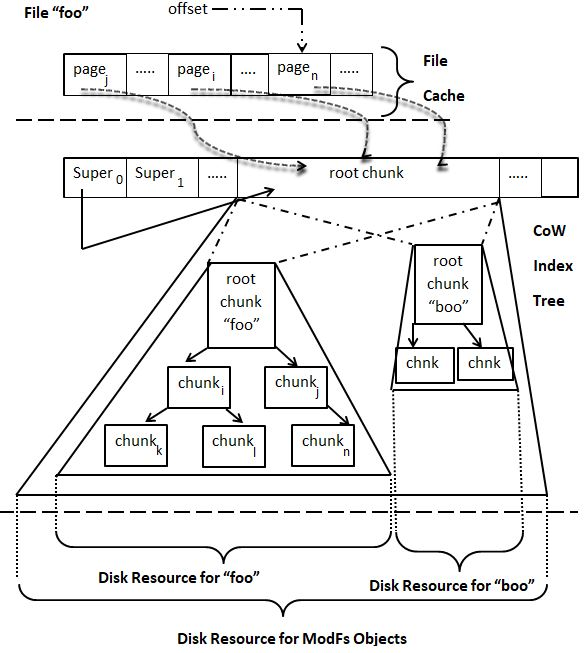
\includegraphics[scale=0.45]{cow_index_tree}
   
    
    \label{fig:placeholder}
\end{figure}
\end{column}

\begin{column}{0.35\textwidth}
\begin{itemize}
    \item An uniquely identifying snapshotting identifier naming the consistent pieces of disk.
    \item Snapshot updates are assumed to be atomic: always have a consistent \emph{view} of the disk-tree
    \item Recovery, Atomicity ....
\end{itemize}
\end{column}

    \end{columns}
\end{frame}
\begin{frame}{Another Example Consistency Model: CoW Filesystems with Snapshots}
\begin{columns}
\begin{column}{0.65\textwidth}  
\begin{figure}
    \centering
    \caption{Depicting Snapshotting Model}
    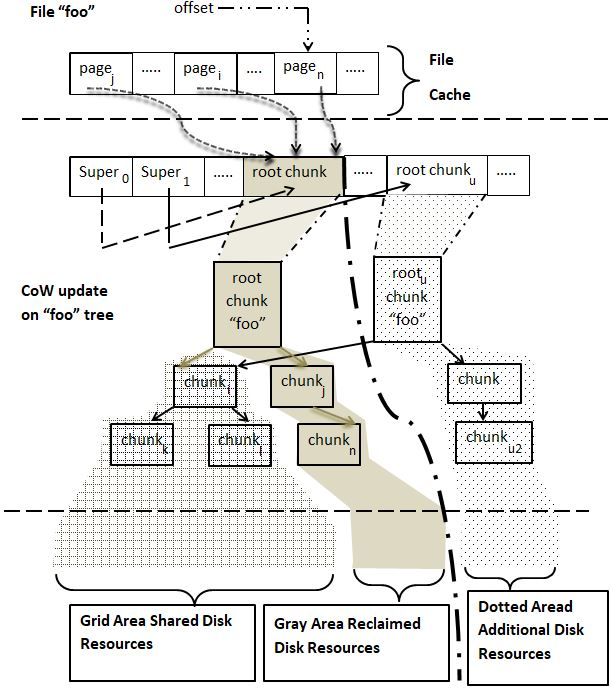
\includegraphics[scale=0.45]{cow_index.png}
   
    
    \label{fig:placeholder}
\end{figure}
\end{column}

\begin{column}{0.35\textwidth}
\begin{itemize}
    \item An uniquely identifying snapshotting identifier naming the consistent pieces of disk.
    \item Snapshot updates are assumed to be atomic: always have a consistent \emph{view} of the disk-tree
    \item Recovery, Atomicity ....
\end{itemize}
\end{column}

    \end{columns}
\end{frame}
\makepart{Logic: Encoding Modalities in Modern Program Logics}
\begin{frame}{Modal Encoding of Hoare Triples for Specifying Programs}
\begin{columns}
    \begin{column}{0.5\textwidth}
    $
    \begin{array}{l}
        \{P\}\; C\; \{Q\} \\ 
        \mathsf{can}\; \mathsf{be}\; \mathsf{encoded}\; \mathsf{in}\; \mathsf{terms}\; \mathsf{of} \\
        P \implies [C] \; Q  \\ \quad \\ \quad\quad\quad\cite{pratt1976semantical}
        
    \end{array}
    $
    \end{column}
    \begin{column}{0.5\textwidth}
        \begin{itemize}
            \item Requires a semantics defined in terms of an underlying semantics
            \begin{itemize}
                \item E.g., Kripke model requires picking up a state, a transition relation between states and a state interpretation function 
            \end{itemize}
            \item Some program logics embed the Kripke explicitly into their models \cite{gordon2019modal} \cite{amalreal2024}
            \end{itemize}
    \end{column}
\end{columns}
   
\end{frame}
\begin{frame}{Modal Encoding of Shallow Modalities for Specifying Programs}
     \begin{itemize}
            \item Some program Logics already utliizes Kripke model deep in their logical machinery \cite{jung15, jung2018iris} which enables lifting these logical machinery for defining other custom-tailored \emph{shallow} modalities
            \item Now we can abuse the notation and read  $[C] \; Q$ as ...  
            \end{itemize}   
\end{frame}
    \scriptsize
    \bibliography{reference.bib}
    \bibliographystyle{ACM-Reference-Format}

%----------------------------------------------------------------------------------------
\end{document}


